\documentclass{report}
%\usepackage[spanish]{babel}
\usepackage[utf8]{inputenc}
\usepackage{parskip}
\usepackage{color}
\usepackage{setspace}
\usepackage{amsmath}
\usepackage{epsfig}
\usepackage{graphicx,multicol}
\usepackage{color}
\usepackage{rotating}

\usepackage{amssymb} 
\usepackage{natbib}
\usepackage{graphicx}
\usepackage[small,bf]{caption}
%\usepackage{txfonts}
\usepackage{hyperref}

\renewcommand{\contentsname}{Indice}
\renewcommand{\listfigurename}{Lista de Figuras}
\renewcommand{\listtablename}{Lista de Tablas}
\renewcommand{\bibname}{Bibliograf\'{\i}a}
\renewcommand{\indexname}{Indice}
\renewcommand{\figurename}{Figura}
\renewcommand{\tablename}{\small Tabla}
\renewcommand{\partname}{Parte}
\renewcommand{\chaptername}{Capítulo}
\renewcommand{\appendixname}{Apéndice}
\renewcommand{\abstractname}{Resumen}




\def \espe  {\text{E}}


%%   
%\def \ecm  {\text{ECM}}

\def \var  {\text{VAR}}
%\def \ses  {\text{SES}}

%% o bien

\def \ecm  {\mbox{\sc ecm}}
\def \var  {\mbox{\sc var}}
\def \ses  {\mbox{\sc ses}}


\renewcommand{\chaptername}{Capítulo}
\renewcommand{\refname}{Bibliografía}




\def\dst{\displaystyle}



%%%%%%%%%%%%%%%%%%%%%%%%%%%%%%%%
% CARATULA
%%%%%%%%%%%%%%%%%%%%%%%%%%%%%%%%
\begin{document}
	\thispagestyle{empty}
	\pagenumbering{roman}
	\setcounter{page}{1}
	
	\begin{center}
		\begin{tabular}{cccccc}
			\hline 
			\hspace{10cm}
		\end{tabular}
		
		\vspace{0.5cm}
		
		\textbf{\Large{
				Regresión logística multinomial en alta dimensión} 
			\vspace{1cm} } 
		
		{\it por}\\
		
		\medskip
		
		Agustín Molina  
		
		
		
		
		\vspace{2cm}
		
		
		TESIS PRESENTADA PARA OPTAR AL TITULO DE \\
		
		{\bf Licenciado en Ciencias de la Computación}
		
		\vspace{1cm}
		
		
		en el
		
		Departamento de Computación 
		
		Facultad de Ciencias Exactas, Físico- Químicas y Naturales
		
		{\bf UNIVERSIDAD NACIONAL DE RIO CUARTO}
		
		\vspace{2cm}
		
		Diciembre de  2024
		
		\vspace{1cm}
		
		\begin{tabular}{cccccc}
			\hline 
			\hspace{10cm}
		\end{tabular}
		\begin{tabular}{cccccc}
			\hline 
			\hspace{10cm}
		\end{tabular}
		
		
		\end {center}
		
		\newpage
		
		\begin{center}
			\vspace{1.5cm}
			\begin{tabular}{cccccc}
				\hline 
				\hspace{10cm}
			\end{tabular}
			
			\vspace{1.5cm}
			
			Tutores:\\
			\medskip
			{\it \textbf{Doctor Marcelo Ruiz}} \\
			
			Departamento de Matemática\\ FCEFQyN, UNRC \\
			
			
			
			
			
			{\it \textbf{ Magister Fabio Zorzán }} \\
			Departamento de Computación\\ FCEFQyN, UNRC \\
			
			\medskip
			
			\medskip
			
			
			
			
			
			\vspace{8cm}
			
			\begin{tabular}{cccccc}
				\hline 
				\hspace{10cm}
			\end{tabular}
			\begin{tabular}{cccccc}
				\hline 
				\hspace{10cm}
			\end{tabular}
			
			
		\end{center}
		
		\newpage
		
		%%%%%%%%%%%%%%%%%%%%%%%%
		% RESUMEN CASTELLANO
		%%%%%%%%%%%%%%%%%%%%%%%
		\newpage
		
		
		\begin{center}
			{\large\textbf{Regresión logística multinomial en alta dimensión}}
		\end{center}
		
		\vspace{2 cm}
		\noindent 
		\section*{Resumen} 		
		
	 
		En esta tesis se desarrolló una herramienta computacional escalable, diseñada para realizar experimentos controlados en la comparación de modelos de clasificación multinomial en contextos de alta dimensión.  Esta herramienta puede adaptarse a la evaluación de bases de datos reales. 
		
		 Más específicamente, abordamos el estudio del desempeño de métodos de estimación del modelo de regresión logística multinomial multiclase.  A través de simulaciones se comparan la regresión logística multinomial clásica con regresión logística con regularización que permite seleccionar variables, tales como las penalidades lasso y red elástica. Además se evalúan otros  métodos de naturaleza distinta como análisis discrimimante lineal y bosques aleatorios.
		
		Esta investigación utiliza diferentes medidas de evaluación de las metodologías de clasificación como la tasa de clasificación errónea,  la precisión y la exahustividad. El trabajo presenta una comparación de los modelos utilizando diferentes configuraciones y parámetros, así como los resultados y el análisis de los mismos, proporcionando una base sólida para futuras investigaciones y aplicaciones en predicción para ciencia de datos. 
		
	
		
		
		\vspace{1cm}
		\noindent \textsl{}
		\section*{Palabras clave} 	
		 
			
		Herramienta computacional especializada. Clasificación multiclase. Alta dimensión.  Regresión logística multinomial. Regularización. Simulación Monte Carlo.   Aprendizaje automático. Ciencia de datos. 
		

 


		
		 
		
		
		%%%%%%%%%%%%%%%%%%%%%%%
		% agradecimientos
		%%%%%%%%%%%%%%%%%%%%%%%
		\newpage
		\section*{Agradecimientos} 
		\begin{spacing}{1.5}{\it  A completar en la versión definitiva... }
			
			
			
			
		\end{spacing}
		
		
		
		%%%%%%%%%%%%%%%%%%%%%%%%%%
		% INDICE
		%%%%%%%%%%%%%%%%%%%%%%%%%%
		\newpage
		\thispagestyle{empty}
		\pagestyle{plain}
		\tableofcontents
		
		\newpage
		\thispagestyle{empty}
		\newpage
		\thispagestyle{empty} \cleardoublepage
		
		\pagestyle{myheadings}
		
		
		
		
		\newpage
		\thispagestyle{empty}
		
		\pagestyle{plain}
		\listoffigures 
		\listoftables 
		
		
		
		\newpage
		\thispagestyle{empty}
		\newpage
		\thispagestyle{empty} \cleardoublepage
		
		\pagestyle{myheadings}
		\pagenumbering{arabic}
		\setcounter{page}{1}
		

\chapter*{Introducción}
\addcontentsline{toc}{chapter}{Introducción}

El aprendizaje automático  y el aprendizaje estadístico \footnote{Machine learning y statistical learning en inglés, respectivamente. Utilizaremos estos términos en ambos idiomas a lo largo del Trabajo Final} son dos aproximaciones complementarias para abordar diversos desafíos planteados en ciencia de datos. 
Dentro de estas áreas, la clasificación forma parte fundamental del aprendizaje estadístico supervisado, cuyo objetivo es alcanzar un buen desempeño en términos de generalización mediante el entrenamiento de una función sobre los datos disponibles que permita realizar predicciones precisas.

Este problema se torna particularmente desafiante en contextos de alta dimensión, cuando el número de muestras de entrenamiento es pequeño en comparación con el número de variables predictoras. En dichos escenarios, las propuestas clásicas tienden a fallar debido a problemas como el sobreajuste y la falta de capacidad para estimar parámetros confiables. Una de las principales estrategias para abordar estas limitaciones es la regularización, que introduce restricciones adicionales en los modelos para mejorar su capacidad de generalización y reducir la complejidad.

El desarrollo de clasificadores efectivos en estos contextos de alta dimensión representa un gran desafío, especialmente cuando el número de variables predictoras supera al número de muestras de entrenamiento.


En el contexto de clasificación, es común encontrarse con la necesidad de estimar probabilidades de que una observación pertenezca a una clase, cuando el número de clases $K$ es grande, basados en una muestra de tamaño $n$ de un vector de variables  características o explicativas de tamaño $p$. 

En \cite{vincent2014} se mencionan varios ejemplos de datos reales.   Una de las bases de datos analizados por los autores es el de la localización de ciertos tipos de cáncer. El conjunto de datos consiste en $p=217$ expresiones génicas- microARNs- obtenidas por la técnica ``bead-based'' provenientes de $n=162$ muestras de tejidos normales y cancerosos.  Aquí la palabra muestra alude a una observación. Las muestras están divididas en 35 clases: 11 clases normales, 16 clases tumorales y 8 clases de líneas celulares tumorales.   El objetivo de esa investigación es proponer un método de clasificación de tal modo que para una nueva observación $\mathbf{x}=(x_1, \ldots, x_{p})$ del vector de expresiones génicas, el estimador asigne una clase.    Los autores para evitar el quiebre de los algoritmos seleccionan sólo las clases normales y tumorales con más de 5 muestras, quedándose con un conjunto de datos más pequeño de 18 clases con 162 muestras. 


%https://github.com/apolitogaga/ML_AmazonReviews/blob/master/Application%20of%20Synergetic%20Neural%20Network%20in%20Online%20Writeprint%20Identification%20.pdf

Otro ejemplo es el  conjunto de datos de reseñas de Amazon que consiste de   10 mil características textuales (incluyendo características léxicas, sintácticas, idiosincráticas y de contenido) extraídas de 1500 reseñas de clientes del sitio web de comercio de Amazon. Las reseñas se recopilaron de  las reseñas de 50 autores, con 50 reseñas por autor. La tarea principal de clasificación es identificar al autor en función de las características textuales.

%Tumor cell line (línea celular tumoral) se refiere a un grupo de células cancerosas que han sido aisladas de un tumor y cultivadas en laboratorio. Estas células tienen la capacidad de crecer y dividirse de manera indefinida bajo las condiciones adecuadas, lo que las convierte en una herramienta útil para investigaciones científicas.



Entre las diferentes metodologías de clasificación, la regresión logística es ampliamente utilizada. No obstante, la estimación de los parámetros en un modelo de regresión logística multinomial presenta el desafío de tener un gran número de parámetros que aumenta linealmente con el número de clases $K$ y el número de variables explicativas $p$ \citep{nibbering2022}.  


En esta modelización cada clase tiene asociada un vector de parámetros que forma parte del modelo lineal que conecta las variables explicativas con la distribución de probabilidad de la clase. Cuando el número de clases o de variables explicativas es grande, el número de parámetros $p$ fácilmente se acerca al número de observaciones $n$. Esto provoca o el quiebre de los algoritmos de estimación o,  el aumento de la tasa de mala clasificación o clasificación errónea (proporción de observaciones mal clasificadas) y dificulta la interpretación de los parámetros.
 


Frente un número $p$ grande y si hay muchos parámetros del componente lineal del modelo que son ceros- es decir, el modelo es ralo- hay varios métodos de regularización propuestos en la literatura. Uno de ellos es muy conocido y se denomina lasso, que es una abreviatura de  ``operador de selección y contracción'', que es una traducción del inglés ``least absolute shrinkage and selection operator''.  Originalmente esta propuesta fue introducida por \cite{tibshi1996} y realiza la selección de variables estimando los parámetros exactamente iguales a cero, de allí el nombre operador de contracción. 

\cite{friedman2010} proponen la utilización de lasso para una regresión logística multinomial. En este mismo trabajo, \cite{friedman2010} usan red elástica (elastic net) que permite ampliar las opciones de penalización, e intenta resolver las dificultades que lasso tiene cuando hay colinealidad entre las variables características.  

\cite{vincent2014} extienden lasso en el modelo de regresión logística multinomial al ``group-lasso'' de \cite{yuan2006}. Este modelo tiene en cuenta la estructura del modelo multinomial y estima los mismos valores de parámetros no nulos en cada vector de parámetros específico de clase. 
 

\cite{nibbering2022} proponen un algoritmo para la estimación de máxima verosimilitud en el modelo de regresión penalizada multiclase, no obstante en su estudio de simulación el número de predictoras $p$ es pequeño.




 En esta tesis realizamos un recorrido por los métodos de clasificación lineal y abordamos el desempeño comparativo de algunos de estos métodos, con especial énfasis en regresión logística multinomial,  cuando el número de variables $p$ y el número de clases $K$ crece, para ciertos escenarios o regímenes.  	 

 Este pasaje por problemas de machine  y statistical learning es un aspecto importante de este trabajo  por el tipo de problemas computacionales que atravesamos y en vistas de comprender la herramienta que propondremos y el objetivo de su desarrollo. Por ejemplo, es importante comprender aspectos claves de algoritmos complejos como descenso por coordenadas y sus variantes utilizado cuando se regulariza en vistas de seleccionar variables del modelo \cite{friedman2010, sarker2021}. Además este tipo de algoritmos con penalización tienen parámetros de penalización que requieren de técnicas específicas de selección como validación cruzada basada en datos. 



 En este trabajo final se desarrolla   una herramienta que permite, dada una va\-riable aleatoria  categórica $G$ ``respuesta'' y un vector aleatorio   $\mathbf{X}=(X_1,\ldots, X_p)^T$  cuyas entradas son ``predictoras'' establecer mediante un escenario de simulación Monte Carlo comparaciones sobre el desempeño de varios métodos de clasificación para diferentes estructuras de la distribución de $\mathbf{X}$ \citep{chen2017, casella2010}.  La comparación necesita que la herramienta compute tanto el error de entrenamiento como el error test y medidas importantes en términos de selección de variables en un contexto de ``alta dimensión''.    Esta  herramienta puede ser de especial utilidad para profesionales de la computación como  de la estadística que en tanto usuarios necesiten  comparar métodos de clasificación sin necesidad de hacer un recorrido teórico sobre los problemas del machine y del statistical learning como realizamos en este trabajo. 


 La herramienta también puede ser adaptada para comparar métodos de clasificación utilizando una base de datos reales.  Este tipo de comparaciones son importantes para especialistas de otros campos como el de genómica, teledetección, medicina, análisis del discurso- sólo para mencionar algunos- donde el problema de clasificación multiclase cobra relevancia. 


 

El esquema del resto de esta tesis es el siguiente. En el Capítulo \ref{reglineal} abordamos el problema de regresión lineal,  dado que  es un antecdente natural de la regresión logística. En el Capítulo \ref{capclasif} hacemos un recorrido por métodos de clasificación lineal, comenzando con el clasificador de Bayes,  análisis discriminante lineal,  regresión logística clásica para finalmente abordar las propuestas de Regresión logística multinomial penalizada.    La estimación del modelo de regresión logística multinomial utilizando un parámetro de penalización se introduce en el Capítulo \ref{capreglogreg}.   En el Capítulo \ref{herramienta} presentamos la estructura del problema de simulación y el desarrollo de la herramienta mencionada. En el Capítulo \ref{reglogmult}  utilizamos la dicha herramienta para realizar un estudio de simulación    a los fines de estudiar el desempeño de los métodos cuando tanto el número de variables predictoras  y el número de clases  crecen y comparamos los métodos en una base de datos reales.  Evaluamos aquí los resultados de un experimento que involucra diferentes escenarios. En el Capítulo \ref{conclus} presentamos las conclusiones principales de esta tesis.


 







\chapter{Regresión lineal}\label{reglineal}


 El modelo de regresión lineal asume la existencia de una relación lineal entre una variable respuesta $Y$ y  un vector $\mathbf{X}=(X_1, \ldots, X_p)$ cuyas entradas son variables predictoras o variables independientes. Al  análisis estadístico de este modelo se lo denomina  (análisis de) regresión lineal. 
 
 La regresión lineal tiene como objetivos el establecer un modelo simple y  estimar a partir de los datos los componentes del modelo en vistas de hacer predicciones de la variable de respuesta para nuevas observaciones de las variables dependientes. 
 
 En el contexto del aprendizaje estadístico este análisis se denomina supervisado, dado que hay una variable respuesta, a la cual se la llama variable de salida. A las variables predictoras se les denomina  variables de entrada o características. 
 
 En este capítulo introducimos principalmente el problema de selección de variables como una consideración preliminar al problema de clasificación del Capítulo \ref{capclasif}.
 

\section{El modelo}




 El modelo de regresión lineal múltiple se define como 
\begin{eqnarray}\label{modelolinealmultiple}
Y=\beta_0+\beta_1X_1+\beta_2 X_2+...+\beta_pX_p+ \epsilon
\end{eqnarray}
donde $Y$ es la variable respuesta, $\mathbf{X}=(X_1, \ldots, X_p)$  es el vector de variables independientes o predictoras, $\beta_1, \ldots, \beta_p$ son los coeficientes del modelo y $\epsilon$ es el término del error, una variable aleatoria con $\espe(\epsilon)=0$ y $\var(\epsilon)=\sigma^2$ finita.   Las variables predictoras pueden ser fijas (controladas) o bien aleatorias.  
Notar que si $\mathbf{X}$ es un vector aleatorio, dado $\mathbf{x}=(x_1, \ldots, x_p)^T$ un vector en $\mathbb{R}^p$, la esperanza condicional  $\espe (Y|\mathbf{X}=\mathbf{x})=\beta_0+\sum_{j=1}^{p}x_j\beta_j$. Si no hay mención contraria, asumiremos que las predictoras son controladas. 


 Para cada $j$, $\beta_j$ cuantifica la asociación entre esa variable y la respuesta; más específicamente representa el efecto promedio sobre $Y$ de un aumento de una unidad en $X_j$, manteniendo todos los demás predictores fijos \citep[p.~72]{james2021}. 


 El objetivo de la regresión lineal es estimar el vector de parámetros $\boldsymbol{\beta}_0^T=(\beta_0,\beta_1,\ldots, \beta_p)$. En general $\sigma^2$ es también desconocido y necesita ser estimado. 


 El modelo \eqref{modelolinealmultiple} se puede escribir en forma compacta como:
\begin{eqnarray}\label{modelolinealmultiplevec}
Y=\mathbf{X}^T \boldsymbol{\beta}_0+ \epsilon,
\end{eqnarray}
donde $\mathbf{X}^T=(1,X_1,\ldots, X_p)$ y $\boldsymbol{\beta}_0^T=(\beta_0,\beta_1,\ldots, \beta_p)$. 




 Consideremos un conjunto de datos $\mathcal{D}$ consistente del vector respuesta $\mathbf{y}=\left(y_1, \ldots, y_n\right)^T \in$ $\mathbb{R}^n$ y una matriz de diseño $\mathbb{X} \in \mathbb{R}^{n \times (p+1)}$ conteniendo $n$ observaciones $\mathbf{x}_i=$ $\left(1,x_{i 1}, \ldots, x_{i p}\right)^T(1 \leq i \leq n)$ de $\mathbf{X}$ y satisfaciendo el modelo \eqref{modelolinealmultiple}:
\begin{eqnarray}\label{modelolinealmultiplen}
y_i=\mathbf{x}_i^T \boldsymbol{\beta}_0+  \epsilon_i, \quad 1 \leq i \leq n
\end{eqnarray}
donde  $\epsilon_1, \ldots, \epsilon_n$ es una muestra aleatoria de $\epsilon$.


 Usualmente la estimación del vector de coeficientes se lleva a cabo  por el método de mínimos cuadrados. Para introducir este método recordemos que,  dado un vector  $\mathbf{z}=(z_1,\ldots,z_n)$,   $\|\mathbf{z}\|_2=(\sum_{j=1}^nz_j^2)^{1/2}$ es la norma 2. Entonces, si definimos, para un vector de parámetros  $\boldsymbol{\beta}_0$ la suma de cuadrados del error (SCE) como:
\begin{eqnarray}\label{sce}
\text{SCE}(\boldsymbol{\beta}_0)&=&\sum_{i=1}^n\left(y_i-\beta_0-\sum_{j=1}^p x_{i j} \beta_j\right)^2\\ 
&=&\|\mathbf{y}-\mathbb{X} \boldsymbol{\beta}_0\|_2^2,\nonumber 
\end{eqnarray}
se define el valor estimado 
\begin{eqnarray}\label{mincuadr}
\widehat{\boldsymbol{\beta}_0}=\text{argmin}_ {\boldsymbol{\beta} \in \mathbb{R}^{p+1}}\text{SCE}(\boldsymbol{\beta}_0)
\end{eqnarray}
si este mínimo existe.  


 Si la matriz $X^TX$ es invertible, entonces la única solución a \eqref{mincuadr} viene dada por:
\begin{eqnarray}\label{mincuadrsolu}
	\widehat{\boldsymbol{\beta}_0}=(\mathbb{X}^T\mathbb{X})^{-1}\mathbb{X}^T\mathbf{y}.
\end{eqnarray}

 De este modo, para una nueva observación $\mathbf{x}_0=\left(1,x_{10}, \ldots, x_{p0}\right)$, el valor predicho por el modelo es:
$$\widehat{y}(\mathbf{x}_0)=\mathbf{x}_0^T	\widehat{\boldsymbol{\beta}_0}.$$


 Si a las suposiciones hechas sobre el modelo agregamos que 
\begin{eqnarray}\label{modelonorm}
\epsilon \sim N(0,\sigma^2)
\end{eqnarray}
entonces es simple demostrar que 
$$
\widehat{\boldsymbol{\beta}_0} \sim N\left(\beta,\left(\mathbb{X}^T \mathbb{X}\right)^{-1} \sigma^2\right)  \text{ y } (n-p-1) \hat{\sigma}^2 \sim \sigma^2 \chi_{n-p-1}^2,$$ 

donde 

$$
\hat{\sigma}^2=\frac{1}{n-p-1} \sum_{i=1}^n\left(y_i-\hat{y}_i\right)^2 
$$
y $\widehat{y}_i=\mathbf{x}_i \widehat{\boldsymbol{\beta}_0}.$  


 Así,  $\widehat{\boldsymbol{\beta}}$ y $\hat{\sigma}^2$ son estimadores insesgados de  $ \boldsymbol{\beta} $ y $ \sigma^2$; el conocimiento de las distribuciones de los estimadores permite construir intervalos de confianza y pruebas de hipótesis \citep{htf}. 


 Es importante notar que en la teoría clásica expuesta hasta aquí, estamos asumiendo que $n>p$, caso contrario $\mathbb{X}^T\mathbb{X}$ no es invertible y por lo tanto  \eqref{mincuadrsolu} no existe.


\section{Selección de variables}
 Escribamos $\boldsymbol{\beta}_0^T=(\beta_0,\boldsymbol{\beta}^T)$ con $\boldsymbol{\beta}^T=(\beta_1,\ldots, \beta_p)$.  Asumiendo que el modelo \eqref{modelolinealmultiple} es válido y si los datos permiten rechazar la hipótesis nula $H_0$: $\boldsymbol{\beta}=\boldsymbol{0}$
entonces el problema qué surge es decidir con qué subconjunto del total de variables $X_1,\ldots, X_p$ nos quedamos.  Es decir, abordamos el problema de la selección del modelo óptimo. 


 Como afirma \cite{christidisthesis}, una condición necesaria pero no suficiente en la  selección de un buen modelo es que prediga bien. Por ejemplo, en el proceso de toma de decisiones de alto riesgo en el sector financiero  necesitamos utilizar un modelo que también sea interpretable. Recientemente, en la literatura han aparecido varios artículos influyentes que lanzan una mirada crítica al uso de algoritmos predictivos tipo ``caja negra'' no interpretables. \cite{christidisthesis} menciona, al igual que otros trabajos allí citados, que los procedimientos estadísticos deben mantener un cierto grado de interpretabilidad a pesar de su alta precisión predictiva.  \cite{rudin2019} enfatizó en los riesgos de utilizar modelos no interpretables y el potencial daño que pueden causar a la sociedad si se aplican en ciertos campos como la atención médica, la visión por computadora o la justicia penal.  \cite{rudin2019} introducen principios fundamentales acerca de las propiedades que debería satisfacer un modelo estadístico interpretable.


 La discusión sobre la interpretabilidad y la fuerza predictiva de un modelo ha cobrado especial relevancia en los últimos años en el contexto de los problemas de alta dimensión, cuando el número de predictoras $p$ es mucho más grande que el número de observaciones $n$,  que denotaremos con $p>>n$. 


 Para datos de alta dimensión es deseable un modelo parsimonioso que incluya un subconjunto con un pequeño número de variables predictoras. 


 En las últimas  décadas y en este contexto se desarrollaron métodos que producen modelos ralos - en los que el vector de coeficientes tiene muchas entradas nulas- que combinan potencia predictiva con buena interpretabilidad. Por extensión, a estos métodos también se los denomina ralos. De modo esquemático, un método ralo optimiza la bondad de ajuste de un modelo restringiendo su complejidad, obteniendo un modelo interpretable con una buena capacidad predictiva  \citep{rudin2019}.


 La aproximación más natural para la modelización rala se denomina selección del mejor subconjunto (BSS), introducida hace mucho tiempo por \cite{gar1965}, y viene dada como solución del siguiente problema no convexo: 
\begin{eqnarray}\label{eq:1.2}
	\min _{\boldsymbol{\beta}_0\in \mathbb{R}^{p+1}}\|\mathbf{y}-\mathbb{X} \boldsymbol{\beta}_0\|_2^2 \quad \text { sujeto  a } \quad\|\boldsymbol{\beta}_0\|_0 \leq t
\end{eqnarray}
donde $\|\boldsymbol{\beta}_0\|_0$ es la norma $\ell_0$ del vector de coeficientes $\boldsymbol{\beta}_0$; i.e. el número de coeficientes no nulos de $\boldsymbol{\beta}_0$. 

%La solución a este problema, es decir  la estimación del coeficiente se produce de modo automático y basado en los datos, como por ejemplo, por convalidación cruzada. 


 Mientras que el procedimiento BSS ha mostrado tener propiedades muy deseables en términos de selección y de propiedades de estimación, la restricción severa es que tiene complejidad NP, dado que hay 
\begin{eqnarray} \label{eq:1.3}
	\mathcal{K}(p, t)=\sum_{j=0}^t\left(\begin{array}{l}
		p \\
		j
	\end{array}\right)
\end{eqnarray}
posibles subconjuntos que deben ser evaluados para determinar la solución óptima. Por ejemplo, $$\mathcal{K}(50,10)=13432735555$$  el cual es un número  muy grande, aun siendo $p$ moderado. 


 Hay diferentes alternativas que reducen la búsqueda a una subclase menor de subconjuntos  como los procedimientos paso a paso ``hacia adelante'' (forward) o ``hacia atrás'' (backward) o mixtos \citep[p.~79]{james2021}. En cada paso, agregan o remueven predictoras del subconjunto vigente basándose en algún tipo de medida de bondad de ajuste hasta que el modelo ya no se pueda mejorar y entonces el procedimiento se detiene. No obstante adolecen de varios inconvenientes \citep{christidisthesis}. 


 Para evitar las restricciones de los métodos paso a paso se desarrollaron metodo\-logías basadas en regularización como Lasso (del inglés ``least absolute shrinkage and selection operator''). Este método resuelve un problema del tipo:
$$
\min _{\boldsymbol{\beta}_0 \in \mathbb{R}^p}\|\mathbf{y}-\mathbb{X} \boldsymbol{\beta}_0\|_2^2 \text { sujeto a  }\|\boldsymbol{\beta}_0\|_1 \leq t
$$
o, en su forma Lagrangiana,
$$
\min _{\boldsymbol{\beta}_0 \in \mathbb{R}^p}\|\mathbf{y}-\mathbb{X} \boldsymbol{\beta}_0\|_2^2+\lambda\|\boldsymbol{\beta}\|_1
$$
donde $\|\cdot \|_1$ es la norma   $\ell_1$ de $\boldsymbol{\beta}$ dada por $$\|\boldsymbol{\beta}\|_1=\sum_{j=1}^p\left|\beta_j\right|.$$ 


 La penalización  $\ell_1$ produce que algunos coeficientes se hagan iguales a cero. A $\lambda \geq 0$  se le llama penalidad lasso y a medida que su valor aumenta provoca que la solución sea un vector $\boldsymbol{\beta}$ más ralo; i.e., con más entradas nulas. El valor de este parámetro del método $\lambda$ es típicamente elegido por validación cruzada. 


 Lasso es utilizado frecuentemente en dominios con grandes cojuntos de datos, en genómica y análisis web \cite{friedman2010}. 

 Sin embargo, lasso posee algunos inconvenientes, tal como lo mencionan \cite{zou2005, friedman2010}:
\begin{itemize}
	\item En la situación en que $n>p$,  para que posea buenas propiedades de selección y para que alcance un error de predicción comparable al de BSS hay que imponer condiciones restrictivas sobre la covarianza de las predictoras.
	\item En el mismo escenario anterior, $n>p$,  si hay un grupo de variables con alta correlación de a pares, lasso tiende a seleccionar sólo una variable del grupo y no hay control sobre cuál selecciona. 
	\item  Y en el escenario usual de alta dimensión, cuando $p>n$,  lasso selecciona a lo sumo $n$ variables, con lo cual es muy limitado.		
\end{itemize}


  En los trabajos de \cite{yuan2006}   y   \cite{meier2008}  se introducen una versión de lasso, denominada lasso por grupos (grouped lasso) que permite en el que las variables son incluidas o excluidas por grupos. 


 Una alternativa a Lasso es la propuesta llamada red elástica  introducida por \cite{zou2005} que resuelve un  problema de la forma: 
\begin{eqnarray}\label{elasnet}
\min _{\boldsymbol{\beta}_0\in \mathbb{R}^{p+1}} R_{\lambda}(\boldsymbol{\beta})
\end{eqnarray}
donde


\begin{eqnarray}\label{elasnetrlam}
 R_{\lambda}(\boldsymbol{\beta}_0)=\frac{1}{2n}\|\mathbf{y}-\mathbb{X} \boldsymbol{\beta}_0\|_2^2+ \lambda P_{\alpha}(\boldsymbol{\beta}), 
\end{eqnarray}
con 
\begin{eqnarray}\label{elasnet2}
P_{\alpha}(\boldsymbol{\beta})=\alpha\|\boldsymbol{\beta}\|_1+\frac{1-\alpha}{2}\|\boldsymbol{\beta}\|_2^2, \
\end{eqnarray}
siendo $\alpha \in [0,1]$ y $\lambda \geq 0.$


 A $P_{\alpha}(\boldsymbol{\beta})$ se le denomina penalización red elástica. Cuando en \eqref{elasnet} hacemos  $\alpha=0$, el método se denomina regresión ridge y si $\alpha=1$ estamos frente a lasso.  La denominación red elástica en un sentido estricto es cuando $\alpha \in (0,1)$.


 Regresión ridge posee el inconveniente que no selecciona variables y lasso es indiferente a la situación de muchas variables correlacionadas, tendiendo a seleccionar una e ignorar las restantes. En el caso extremo de $k$ predictoras idénticas el método se rompe \citep{friedman2010}. 


 Red elástica es particularmente útil cuando $p \gg n$, además permite seleccionar hasta  $p$ predictoras (provisto que $\alpha < 1$ ) y, tiene  un buen desempeño aún cuando haya muchas variables correlacionadas. 


 \cite{zou2006} introdujo un método denominado lasso adaptivo  que tiene propiedades óptimas de oráculo. A saber, identifica el subconjunto correcto del modelo, $\mathcal{A}=\left\{j: \hat{\beta}_j \neq 0\right\}$ y, además tiene una tasa óptima de convergencia en distribución $$\sqrt{n}\left(\hat{\boldsymbol{\beta}}_{\mathcal{A}}-\boldsymbol{\beta}_{\mathcal{A}}^*\right) \rightarrow_d\mathrm{N}\left(\mathbf{0},  \Sigma^*\right),$$ donde $ \Sigma^*$ es la matriz de covarianza del verdadero modelo.

 No obstante, para obtener un buen desempeño predictivo el autor recomienda utilizar el estimador de ridge (el caso $\alpha = 0$) cuando  hay predictoras altamente correlacionadas. 


 
 \section{Algoritmos de regularización}
 
 
 En esta sección seguimos la exposición de \cite{htw}, Capítulo 2.  
 Por simplicidad asumiremos que  en el modelo de regresión lineal múltiple \eqref{modelolinealmultiplen} $\beta_0=0$ y que  las observaciones están estandarizadas:
 \begin{eqnarray}\label{estand}
 \sum_{i=1}^n x_{i j}=0, \frac{1}{n} \sum_{i=1}^n x_{i j}^2=1 \text {, para } j=1, \ldots, p \text {. }
 \end{eqnarray}


 Vamos a estudiar el problema de lasso, es decir que en \eqref{elasnet} consideramos $\alpha=1$


 El problema lasso consiste entonces en resolver, para un $\lambda$ dado: 
\begin{eqnarray}\label{lasso}
\min _{\boldsymbol{\beta} \in \mathbb{R}^{p}} R_{\lambda}(\boldsymbol{\beta})= \underset{\boldsymbol{\beta} \in \mathbb{R}^p}{\operatorname{min}}\left\{\frac{1}{2n} \sum_{i=1}^n\left(y_i-\sum_{j=1}^p x_{i j} \beta_j\right)^2+\lambda \sum_{j=1}^p\left|\beta_j\right|\right\} \text {. }
\end{eqnarray}

 
 Dividimos la estrategia de solución en dos casos, cuando hay un único predictor o cuando hay más de uno.  
 

\subsubsection*{Optimización lasso cuando el predictor es único}


 Supongamos que el modelo tiene un único predictor y así nuestra muestra tiene la forma $\{(z_i,y_i)\}_{i=1}^n$, donde hemos renombrado $z_i=x_{ij}$. De este modo el problema a resolver es 
$$
\min _{\beta \in \mathbb{R}} \left\{\frac{1}{2 n} \sum_{i=1}^n\left(y_i-z_i \beta\right)^2+\lambda|\beta|\right\} \text {. }
$$


 La estrategia típica es hallar el punto crítico de la función a minimizar derivando, pero el problema es que la función objetivo no es derivable en $\beta=0$. De todos modos, por inspección directa probamos que
$$
\widehat{\beta}= \begin{cases}\frac{1}{N}\langle\mathbf{z}, \mathbf{y}\rangle-\lambda & \text { si  } \frac{1}{n}\langle\mathbf{z}, \mathbf{y}\rangle>\lambda, \\ 0 & \text { si } \frac{1}{n}  \rvert\,\langle\mathbf{z}, \mathbf{y}\rangle \rvert\ \leq \lambda, \\ \frac{1}{n}\langle\mathbf{z}, \mathbf{y}\rangle+\lambda & \text { si  } \frac{1}{n}\langle\mathbf{z}, \mathbf{y}\rangle<-\lambda \end{cases}
$$

donde 

$\mathbf{z}^T=(z_1,\ldots,z_n)$ e  $\mathbf{y}^T=(y_1,\ldots,y_n)$ y $\langle\mathbf{z}, \mathbf{y}\rangle>$ denota el producto interno de ambos vectores. 


Si definimos el operador (de soft-thresholding en inglés) definido sobre $\mathbb{R}$
$$
\mathcal{S}_\lambda(x)=\operatorname{sign}(x)(|x|-\lambda)_{+},
$$


entonces podemos escribir en forma compacta:
$$ \widehat{\beta}= \mathcal{S}_\lambda(\frac{1}{n}\langle\mathbf{z}, \mathbf{y}\rangle).$$


\subsubsection*{Optimización lasso con predictores múltiples: descenso por coordenadas }


 Nos basaremos en el desarrollo que se llevó a cabo cuando hay un único predictor. 


 La estrategia consiste en recorrer cíclicamente los predictores en algún orden fijo (pero arbitrario), por ejemplo $j=1, \ldots, p$ de tal modo que en el $j$-ésimo paso actualizamos el coeficiente $\beta_j$ minimizando la función objetivo en esta coordenada manteniendo fijos los otros coeficientes $\{\widehat{\beta}_j, j\neq k\}$ en sus valores actuales.


 Si escribimos \eqref{lasso} como 
$$
\frac{1}{2 n} \sum_{i=1}^n\left(y_i-\sum_{k \neq j} x_{i k} \beta_k-x_{i j} \beta_j\right)^2+\lambda \sum_{k \neq j}\left|\beta_k\right|+\lambda\left|\beta_j\right|
$$
es claro que la solución para cada $\beta_j$ se puede escribir en términos del residuo parcial 
$$r_i^{(j)}=y_i-\sum_{k\neq j}x_{ik}\widehat{\beta}_k.$$ 


 Este residual remueve del valor observado $y_i$ el ajuste actual de todas las predictoras excepto la $j$-ésima. En términos del residuo parcial, el $j$-ésimo coeficiente es actualizado por 
\begin{eqnarray}\label{actua}
\widehat{\beta}_j= \mathcal{S}_\lambda(\frac{1}{n}\langle\mathbf{x}_j, \mathbf{r}^{(j)}\rangle) 
\end{eqnarray}
con $\mathbf{r}^{(j)}=(r_1^{(j)}, \ldots, r_p^{(j)})^T$.


 Equivalentemente, como 
$$ \widehat{\beta}_j \leftarrow \mathcal{S}_\lambda( \widehat{\beta}_j+ \frac{1}{n}\langle\mathbf{x}_j, \mathbf{r}\rangle)$$

donde 

$\mathbf{r}^T=(r_1,\ldots,r_p)$ y  $r_i=y_i-\sum_{j=1}^p x_{i j} \widehat{\beta}_j$, $i=1,\ldots, p$.


 El algoritmo opera aplicando la actualización \eqref{actua} repetidamente de modo cíclico, actualizando las coordenadas de $\widehat{\boldsymbol{\beta}}$ a lo largo del camino elegido. 
 

 La convergencia está garantizada ya que la función a minimizar en \eqref{lasso} es convexa sin mínimos locales. El algoritmo introducido se denomina descenso cíclico por coordenadas, y minimiza la función objetivo  por coordenada, de a una a la vez. Bajo condiciones débiles la minimización coordenada a coordenada converge al mínimo global. 
 
 
  
   
 
   
 
 
 

\chapter{Métodos lineales de clasificación}\label{capclasif}


 Consideremos el problema de predecir una respuesta  categórica $G$ utilizando múltiples predictores. Como sinónimo de variable aleatoria categórica algunos autores utilizan la palabra  factor \cite{htf}. 
En lugar de predicción, en este contexto se utiliza más comúnmente el término clasificación.


 Ejemplos típicos son-  en morfología vegetal-  la clasificación de especies  a partir de ciertas características de la flor o - en  análisis de imágenes-  la identificación de los números en un código postal escrito a mano a partir de una imagen digitalizada.  


 Más específicamente, $G$ es una variable aleatoria que asume valores en un conjunto finito ${\cal G}$ que, sin pérdida de generalidad podemos asumir  ${\cal G}=\{1, \ldots, K\}$. Como antes, sea  $\mathbf{X}=(X_1,\ldots, X_p)^T$ un vector aleatorio cuyas entradas- las variables predictoras- se denominan también características (inputs en inglés). 

 Un clasificador  es una regla de clasificación  $\widehat{G}$ que a cada valor $\mathbf{x}$ de $\mathbf{X}$ le asigna una clase, $\widehat{G}(\mathbf{x})$ en ${\cal G}$ \citep{devroye1996}.  Un error ocurre cuando 
 $\widehat{G}(\mathbf{x})\neq G$ y la probabilidad de error del clasificador se define como
 \begin{eqnarray}\label{proberror}
 L=P(\widehat{G}(\mathbf{X})\neq G).	 
 \end{eqnarray}

 
 El clasificador de Bayes se define como:
 \begin{eqnarray}\label{clasBayes}
G_B(\mathbf{x})=k \text { si y sólo si } P\left(G=k \mid \mathbf{X}=\mathbf{x}\right)=\max _{j \in \mathcal{G}} P(G=j \mid \mathbf{X}=\mathbf{x}).
 \end{eqnarray}
 Es decir, asignamos la clase más probable utilizando la distribución condicional $P\left(G  \mid \mathbf{X} \right).$   La tasa de error o tasa de mal clasificación de este clasificador es llamada la tasa de Bayes \citep[p.~21]{htf}. Para una introducción más formal al problema general de clasificación ver \cite{bousquet}. 
 	
 	
 
 Para utilizar la regla de clasificación dada en \eqref{clasBayes}, como  las probabilidades a posteriori $P(G=j \mid \mathbf{X}=\mathbf{x})$ son desconocidas   tienen que ser estimadas. Los métodos de clasificación que presentaremos abordan el problema de construir estimadores de estas probabilidades.
 
  Supongamos, como en el Capítulo 4 de  \cite{htf}, que $f_k(x)$ es la densidad de la distribución condicional de $\mathbf{X}$ en la clase  $G=k$, y sea $\pi_k$ la probabilidad a priori de la clase $k$, con $\sum_{k=1}^K \pi_k=1$. Por el Teorema de Bayes 
\begin{eqnarray}\label{clasBayesden}
P(G=k \mid X=x)=\frac{f_k(x) \pi_k}{\sum_{l=1}^K f_{l}(x) \pi_{l}}.
\end{eqnarray}

Algunas  reglas de clasificación están basadas en ciertos supuestos sobre estas  densidades. Por ejemplo \citep{htf}: 
\begin{itemize}
	\item El análisis discriminante lineal   y cuadrático  se basan en densidades Gaussianas.
	\item  Métodos más flexibles que los dos anteriores permiten utilizar mixturas de densidades Gaussianas.
	\item Los métodos no paramétricos usan estimadores estimadores no paramétricos de la densidad.
\end{itemize}


\section{Análisis discriminante lineal}\label{seclda}

En el análisis discriminante lineal (LDA) se asume que las densidades para cada clase son Gaussianas multivariadas  

$$
f_k(\mathbf{x})=\frac{1}{(2 \pi)^{p / 2}\left|\Sigma_k\right|^{1 / 2}} \text{e}{-\frac{1}{2}\left(\mathbf{x}- \boldsymbol{\mu}_k\right)^T \Sigma_k^{-1}\left(\mathbf{x}-\boldsymbol{\mu}_k\right)},\; k=1\ldots, K,
$$
y, además que 
\begin{eqnarray}\label{homog}
\forall k=1,\ldots, K:\;  \Sigma_k=\Sigma;
\end{eqnarray}
es decir, las matrices de covarianza en cada clase son iguales. 

Consideremos el  cociente $$P(G=k \mid\mathbf{X}=\mathbf{x})/ P(G=l \mid \mathbf{X}=\mathbf{x}), $$ al que le llamaremos (en inglés) odds y a su logaritmo log-odds o log-ratio. 

Bajo el supuesto \eqref{homog}   se obtiene:

\begin{eqnarray}\label{logoddsnormal}
		\log \left( \frac{P(G=k \mid\mathbf{X}=\mathbf{x})}{P(G=l \mid \mathbf{X}=\mathbf{x})}\right)&= & \log \left(\frac{\pi_k}{\pi_{l}}\right)-\frac{1}{2}\left(\boldsymbol{\mu}_k+\boldsymbol{\mu}_{l}\right)^T \Sigma^{-1}\left(\boldsymbol{\mu}_k-\boldsymbol{\mu}_{l}\right) \nonumber \\  
& +&\mathbf{x}^T \Sigma^{-1}\left(\boldsymbol{\mu}_k-\boldsymbol{\mu}_{l}\right).
\end{eqnarray}
 

 

Notar que el hecho de que el log-odds sea lineal en $\mathbf{x}$ implica que la frontera de decisión entre las dos clases $k$ y $l$ - es decir el conjunto en el que 
$P(G=k \mid\mathbf{X}=\mathbf{x})=P(G=l \mid\mathbf{X}=\mathbf{x})$- es lineal en $\mathbf{x}$, lo que significa  que en dimensión $p>1$ es un hiperplano.
 

 

Para cada $k=1, \ldots, K$ definamos la función $\delta_k:\mathbb{R}^p\rightarrow \mathbb{R}$ como
$$  
\delta_k(\mathbf{x})=\mathbf{x}^T \Sigma^{-1} \boldsymbol{\mu}_k-\frac{1}{2} \boldsymbol{\mu}_k^T \Sigma^{-1} \boldsymbol{\mu}_k+\log \pi_k.
$$
A cada $\delta_k$ se le denomina función discriminante lineal y, es posible probar que
 \begin{eqnarray}\label{clasBayeslda}
G_B(\mathbf{x})=k \text { si y sólo si } \delta_k(\mathbf{x})=\max _{j \in \mathcal{G}}  \delta_j(\mathbf{x}).
\end{eqnarray}

Desde un punto de vista práctico como no se conocen los parámetros de las distribuciones multivariadas Gaussianas, los estimamos del siguiente modo. Si  $(\mathbf{x}_i, g_i)$, $i=1,\ldots n$ es una muestra de tamaño $n$ del par $(\mathbf{X}, G)$ donde $g_i$ denota la clase correspondiente a la $i$-ésima observación $\mathbf{x}_i=(x_{i,1}, \ldots x_{i,p})^T$ del vector  $\mathbf{X}$, $n_k$ denota el número de observaciones en la clase $k$ y  $n$ el número total de observaciones entonces definimos los siguientes estimadores: 

\begin{eqnarray}\label{clasBayesldaesti}
\hat{\pi}_k&=& n_k / n,\nonumber \\
\hat{\boldsymbol{\mu}}_k &=& \sum_{g_i=k} \mathbf{x}_i / n_k,  \\ 
\hat{\Sigma} &=& \sum_{k=1}^K\sum_{g_i=k}\left(\mathbf{x}_i-\hat{\boldsymbol{\mu}}_k\right)\left(\mathbf{x}_i-\hat{\boldsymbol{\mu}}_k\right)^T /(n-K). \nonumber
\end{eqnarray}

Y finalmente,  las funciones discriminantes lineales estimadas $\widehat{\delta}_k$ que se obtienen reemplazando los parámetros por su estimadores dados en \eqref{clasBayesldaesti} conducen  a la regla de Bayes estimada, denotada por $\widehat{G}_B$. 


Por ejemplo, para dos clases, la regla elige la clase 2 si 

$$\mathbf{x}^T \hat{\Sigma}^{-1}\left(\hat{\boldsymbol{\mu}}_2-\hat{\boldsymbol{\mu}}_1\right)>\frac{1}{2} \hat{\boldsymbol{\mu}}_2^T \hat{\Sigma}^{-1} \hat{\boldsymbol{\mu}}_2-\frac{1}{2} \hat{\boldsymbol{\mu}}_1^T \hat{\Sigma}^{-1} \hat{\boldsymbol{\mu}}_1+\log \left(n_1 / n\right)-\log \left(n_2 / n\right).$$


%ver https://cienciadedatos.net/documentos/28_linear_discriminant_analysis_lda_y_quadratic_discriminant_analysis_qda#An%C3%A1lisis_discriminante_lineal


\section{Regresion logística}


La regresión logística modela las probabilidades a posteriori de las $K$ clases utilizando funciones lineales del vector de variables características. Si bien esta modelización fue introducida hace ya varias décadas, cobró actualidad dada la posibilidad de utilizar propuestas recientes de selección de variables en el contexto de alta dimensión.  Para una aproximación histórica a la regresión logística y su relación con LDA ver la monografía de \cite{cox1970} y el artículo de \cite{efron1975}. 

 


\subsection{Regresion logística binomial}


Para simplificar el abordaje a la regresión logística iniciamos con dos clases, es decir  ${\cal G} = \{1,2\}$. La siguiente modelización de las probabilidades a posteriori  asume que la relación  entre las probabilidades a posteriori y el vector de variables explicativas $\mathbf{X}$ viene dada por:
\begin{eqnarray}\label{logistica2}
 P(G=1 \mid  \mathbf{X}=\mathbf{x})	&=&\frac{\exp \left(\beta_0+\mathbf{x}^T\boldsymbol{\beta} \right)}{1+\exp \left(\beta_0+\mathbf{x}^T\boldsymbol{\beta}\right)}\\
 P(G=2 \mid \mathbf{X}=\mathbf{x})&=& \frac{1}{1+\exp \left(\beta_0+\mathbf{x}^T\boldsymbol{\beta} \right)}\nonumber  
\end{eqnarray}

donde  $\mathbf{x}=(x_1,\ldots, x_p)^T$ y   $\boldsymbol{\beta}=(\beta_1,\ldots, \beta_p)^T$. 


 Utilizando la transformación denominada logit  $g(p)=\log(p/(1-p))$ definida sobre el intervalo $(0,1)$, podemos escribir el log-odds 
\begin{eqnarray}\label{logistica2equiv}
	 \log\left(\frac{P(G=1 \mid  \mathbf{X}=\mathbf{x})}{P(G=2 \mid  \mathbf{X}=\mathbf{x})}\right)=\beta_0+\beta_1X_1+...+\beta_pX_p.
\end{eqnarray}
como una combinación lineal de las entradas de $\mathbf{X}$. 



A este modelo \eqref{logistica2} (o en su formulación equivalente \eqref{logistica2equiv}) se lo llama de modelo de regresión logística binomial multivariado. 

Como afirma \cite{htf} en la Sección 4.4., este modelo es muy utilizado en aplicaciones a la bioestadística  en las cuales la respuesta es binaria. Por ejemplo los pacientes sobreviven o mueren, tienen insuficiencias cardíacas o no, cierta condición está presente o ausente. 


Si llamamos 

\begin{eqnarray}\label{lamb}
	\lambda(\mathbf{x})=\beta_0+\mathbf{x}^T\boldsymbol{\beta}
\end{eqnarray}

entonces teniendo en cuenta las expresiones de las probabilidades condicionales dadas en    \eqref{logistica2}  la regla de decisión se expresa como:

\begin{eqnarray}\label{clasBayes2log}
	G_B(\mathbf{x})=1 \text { si } \lambda(\mathbf{x})>0   \text { y } 	G_B(\mathbf{x})=2  \text { si }  \lambda(\mathbf{x})<0. 
\end{eqnarray}




Si estimamos los coeficientes del modelo \eqref{logistica2equiv} podemos contar con estimaciones de las probabilidades a posteriori \eqref{logistica2} y a partir de \eqref{clasBayes} contar con una regla de clasificación. 



Sea   $(\mathbf{x}_i, g_i)$, $i=1,\ldots n$ una muestra de tamaño $n$  de $(\mathbf{X}, G)$. En la Sección \ref{estimamrlmulti} estudiaremos cómo se obtiene un estimador de $(\beta_0, \boldsymbol{\beta})$ maximizando la función de máxima verosimilitud condicional 
\begin{eqnarray}\label{verosimil1}
	f(g_1,\ldots, g_n|\mathbf{x}_1,\ldots, \mathbf{x}_n )= \prod_{i=1}^n \frac{\exp  \left(\beta_0+ \boldsymbol{\beta}^{\prime} \mathbf{x}_i\right) g_i }{\left[1+\exp \left(\beta_0+ \boldsymbol{\beta}^{\prime} \mathbf{x}_i\right)\right]}
\end{eqnarray}
respecto de $(\beta_0, \boldsymbol{\beta})$. 

Si  $ \bar{\beta}_0$ y $ \bar{\boldsymbol{\beta}}$ denotan los estimadores entonces $\widehat{\lambda}(\mathbf{x})=\bar{\beta}_0+\bar{\beta}^{\prime} \mathbf{x}$ es un estimador de $\lambda$,  y la regla estimada elige la clase 1 cuando $\widehat{\lambda}(\mathbf{x})>0$ y la clase 2 cuando $\widehat{\lambda} (\mathbf{x})<0$.  

%Notar que $\widehat{\lambda}$ es un estimador de la función discriminante lineal. 


\subsection{Relación entre la regresion logística binomial y el LDA}


  \cite{efron1975}  comparó el desempeño del análisis discriminante lineal con el de la regresión logística. 
  
  %Esta comparación nos interesa porque nos va a permitir introducir diferentes escenarios de simulación que son importantes para el desarrollo de esta tesis. 

 

Como en la Sección \ref{seclda} consideremos que el vector de características $\mathbf{X}^T=(X_1,\ldots, X_p)$ puede tener alguna de las dos distribuciones normales multivariadas:
\begin{eqnarray}\label{modelonormalclases}
\mathbf{X}\sim N(\boldsymbol{\mu}_1,\Sigma ) && \text{ con probabilidad } \pi_1\\
\mathbf{X}\sim N(\boldsymbol{\mu}_2,\Sigma ) && \text{ con probabilidad } \pi_2 \nonumber 
\end{eqnarray}
y $\pi_1+\pi_2=1$. 


Sea $\lambda_l: \mathbb{R}^p\rightarrow  \mathbb{R}$ la función 
\begin{eqnarray*}
\lambda_l(\mathbf{x})=\beta_0+\mathbf{x}^T \boldsymbol{\beta}
\end{eqnarray*}
donde 

\begin{eqnarray*}
\beta_0 &=&\log \left( \frac{\pi_1}{\pi_2}\right) -\frac 12 \left( \boldsymbol{\mu}_1^T \Sigma^{-1} \boldsymbol{\mu}_1- \boldsymbol{\mu}_2^T \Sigma^{-1} \boldsymbol{\mu}_2 \right)\\
\boldsymbol{\beta} &=&  \Sigma^{-1}(\boldsymbol{\mu}_2-\boldsymbol{\mu}_1).
\end{eqnarray*}






Si $\mathbf{x}$ es una observación de  $\mathbf{X}$ la regla de decisión para LDA dada en \eqref{clasBayes} se puede expresar como 
\begin{eqnarray}\label{clasBayes2}
	G_B(\mathbf{x})=1 \text { si } \lambda_l(\mathbf{x})>0   \text { y } 	G_B(\mathbf{x})=2  \text { si }  \lambda_l(\mathbf{x})<0. 
\end{eqnarray}

Utilizando los estimadores dados en \eqref{clasBayesldaesti} se obtiene $\widehat{\lambda}_l$, una estimación de  $\lambda_l$ y su correspondiente regla de clasificación. 


Por otro lado, podríamos considerar la estimación $\widehat{\lambda}(\mathbf{x})=\bar{\beta}_0+\bar{\beta}^{\prime} \mathbf{x}$
introducida en el análisis de regresión logística. 




 \cite{efron1975} computa la eficiencia relativa asintótica de los dos procedimientos y muestra que la regresión logística es  mucho menos efectiva que el LDA. En términos más simples, cuando $n$ es grande la tasa de error de la regresión logística es mayor que la de LDA. 


Este resultado se debe a que mientras la regresión logística se basa en la distribución condicional, el análisis discriminante lineal está basado en el estimador de máxima verosimilitud ``completo''.




\subsection{Regresion logística multinomial}


 El modelo de regresión logística binomial se puede generalizar a más de dos clases del siguiente modo: 
\begin{eqnarray} 
	P(G=k \mid  \mathbf{X}=\mathbf{x})	&=&\frac{\exp \left(\beta_{k0}+\mathbf{x}^T\boldsymbol{\beta}_k \right)}{1+\sum_{l=1}^{K-1} \exp \left(\beta_{l 0}+\mathbf{x}^T\boldsymbol{\beta}_{l} \right)}, \; k=1\ldots, K-1\nonumber \\
	P(G=K \mid \mathbf{X}=\mathbf{x})&=& \frac{1}{1+\sum_{l=1}^{K-1} \exp \left(\beta_{l 0}+\mathbf{x}^T\boldsymbol{\beta}_{l} \right)}\label{logisticamult} 
\end{eqnarray}

donde  $\mathbf{x} = (x_1,\ldots, x_p)^T$ y los coeficientes del modelo son $(\beta_{l0}, \boldsymbol{\beta}_{l}^T)$ con $\boldsymbol{\beta}_l^T = (\beta_{l1}, \ldots, \beta_{lp})$, $l = 1, \ldots, K-1$.

 Y de modo análogo a cuando la variable respuesta es binaria, escribimos para la variable multinomial $G$ con $K$ clases:
\begin{eqnarray}\label{logisticamultequiv}
	\log\left(\frac{P(G=k \mid  \mathbf{X}=\mathbf{x})}{P(G=K \mid  \mathbf{X}=\mathbf{x})}\right)=\beta_{k0}+\sum_{l=1}^p\beta_{kl}x_l,\; k=1,\ldots, K-1.
\end{eqnarray}


 Así, el modelo está especificado en términos de los $K-1$ log de los odds o transformaciones logits  y, es irrelevante utilizar como denominador la $K$-ésima clase (podría haber sido cualquier otra clase). 

 A este modelo  se lo llama modelo de regresión logística multinomial multivariada.  De aquí en más le llamaremos modelo de regresión logística binomial o multinomial, omitiendo el término multivariado. 
 
 
\subsection{Estimación clásica del modelo de regresion logística multinomial}\label{estimamrlmulti}


 Escribamos $$ \boldsymbol{\beta}^T=\left(\beta_{10}, \beta_1^T, \ldots, \beta_{(K-1) 0}, \beta_{K-1}^T\right),$$ y denotamos las  probabilidades a posteriori con $$p_k(x ; \boldsymbol{\beta})=P(G=k \mid \mathbf{X}=\mathbf{x})$$
Notar que para simplificar la notación estamos incluyendo en el vector $\boldsymbol{\beta}$ los coeficientes que representan las ordenadas al origen $\beta_{k0}$. 

 Ajustaremos el modelo de regresión logística por máxima verosimilitud, utilizando la ditribución multinomial con parámetros  $p_k(x ; \boldsymbol{\beta})$, $k=1,\ldots, K$.
 

 Luego 
%la función de verosimilitud es $P(N_1=n_1, \ldots, N_K=n_K) $ y, 
la función de log-verosimilitud se puede escribir como: 
\begin{eqnarray}\label{logvero}
\ell(\boldsymbol{\beta})=\sum_{i=1}^N \log p_{g_i}\left(\mathbf{x}_i ; \boldsymbol{\beta}\right).
\end{eqnarray}


 El objetivo es hallar
$$\widehat{\boldsymbol{\beta}}=\text{argmax}_{\boldsymbol{\beta} \in \mathbb{R}^{(p+1)\times (K-1)}} \ell(\boldsymbol{\beta}).$$

 Para simplificar asumiremos que $K=2$, el caso general se aborda en el Apéndice A. Asumamos ademas que las dos clases $g_i$ se pueden escribir como $0$ o $1$ definiendo como respuesta $y_i$, con $y_i=1$ si $g_i=1$, e $y_i=0$ cuando $g_i=2$.  Sea $\boldsymbol{\beta}^T=\left(\beta_{10}, \boldsymbol{\beta}_1^T\right)$ con  
$$\boldsymbol{\beta}_1^T=(\beta_{11}, \ldots, \beta_{1p})$$
y re-escribimos por abuso de notación $$\mathbf{x}_i^T=(x_{i0},x_{i1}, \ldots, x_{ip}),\, \text{ con } x_{i0}=1.$$  Dado $\mathbf{x}$, contamos con dos probabilidades a posteriori
\begin{eqnarray}\label{posteri}
p_1(\mathbf{x} ; \boldsymbol{\beta})=p(\mathbf{x} ; \boldsymbol{\beta}), \text{ y } p_2(\mathbf{x} ; \boldsymbol{\beta})=1-p(\mathbf{x} ; \boldsymbol{\beta})
\end{eqnarray}

Luego, 
\begin{eqnarray}\label{lbeta}
	\begin{aligned}
		\ell(\boldsymbol{\beta}) & =\sum_{i=1}^n\left\{y_i \log p\left(\mathbf{x}_i ; \boldsymbol{\beta}\right)+\left(1-y_i\right) \log \left(1-p\left(\mathbf{x}_i ; \boldsymbol{\beta}\right)\right)\right\} \\
		& =\sum_{i=1}^n\left\{y_i \boldsymbol{\beta}^T \mathbf{x}_i-\log \left(1+\text{e}^{\boldsymbol{\beta}^T \mathbf{x}_i}\right)\right\}
	\end{aligned}
\end{eqnarray}



 Para la maximización hallamos los puntos críticos igualando las derivadas a cero, obteniendo las siguientes $p+1$ ecuaciones no lineales en $\boldsymbol{\beta}$:
\begin{eqnarray}\label{4.21}
	\frac{\partial \ell(\boldsymbol{\beta})}{\partial \boldsymbol{\beta}}=\sum_{i=1}^n \mathbf{x}_i\left(y_i-p\left(\mathbf{x}_i ; \boldsymbol{\beta}\right)\right)=0,
\end{eqnarray}


 Utilizando \eqref{lbeta}:
\begin{eqnarray*}\label{lbeta0}
	0=\frac{\partial \ell(\boldsymbol{\beta})}{\partial \beta_{10}} 	&=& \frac{\partial \ell(\boldsymbol{\beta})}{\partial \beta_{10}} \sum_{i=1}^N\left\{y_i \boldsymbol{\beta}^T \mathbf{x}_i-\log \left(1+\text{e}^{\boldsymbol{\beta}^T \mathbf{x}_i}\right)\right\}\\
	&=& \frac{\partial \ell(\boldsymbol{\beta})}{\partial \beta_{10}} \sum_{i=1}^n\left\{y_i \sum_{j=0}^{p}\beta_{1j} x_{ij}-\log \left(1+\text{e}^{\boldsymbol{\beta}^T \mathbf{x}_i}\right)\right\}\\
	&=&  \sum_{i=1}^n y_i  x_{i0}- \frac{x_{i0}\text{e}^{\boldsymbol{\beta}^T \mathbf{x}_i}}{1+\text{e}^{\boldsymbol{\beta}^T \mathbf{x}_i}}\\
	&=&  \sum_{i=1}^n  x_{i0} \left( y_i - \frac{\text{e}^{\boldsymbol{\beta}^T \mathbf{x}_i}}{1+\text{e}^{\boldsymbol{\beta}^T \mathbf{x}_i}} \right)\\
	&=& \sum_{i=1}^n  x_{i0} \left( y_i - p\left(\mathbf{x}_i ; \boldsymbol{\beta}\right)  \right). 
\end{eqnarray*}
y como $x_{i0}=1$ entonces  la igualdad se reduce a $\dst \sum_{1=1}^n y_i=\sum_{i=1}^n p\left(\mathbf{x}_i ; \boldsymbol{\beta}\right)$.  Análogamente, para cada $j=1,\ldots, p$, 
\begin{eqnarray*}\label{lbetaj}
	0=\frac{\partial \ell(\boldsymbol{\beta})}{\partial \beta_{1j}} 	
	&=& \sum_{i=1}^n  x_{ij} \left( y_i - p\left(\mathbf{x}_i ; \boldsymbol{\beta}\right)  \right). 
\end{eqnarray*}


 Para resolver las ecuaciones \eqref{4.21}, podemos utilizar el algoritmo de Newton-Raphson, el cual requiere hallar la matriz Hessiana 
$$
\frac{\partial^2 \ell(\boldsymbol{\beta})}{\partial \boldsymbol{\beta}  \boldsymbol{\beta}^T}=-\sum_{1=1}^n \mathbf{x}_i \mathbf{x}_i^T p\left(\mathbf{x}_i ; \boldsymbol{\beta}\right)\left(1-p\left(x_1 ; \boldsymbol{\beta}\right)\right) 
$$

 Comenzando con $\boldsymbol{\beta}^{\text {viejo }}$, una actualización simple del algoritmo es la siguiente:
$$
\boldsymbol{\beta}^{\text {nuevo }}=\boldsymbol{\beta}^{\text {viejo }}-\left(\frac{\partial^2 \ell(\boldsymbol{\beta})}{\partial \boldsymbol{\beta} \partial \boldsymbol{\beta}^T}\right)^{-1} \frac{\partial \ell(\boldsymbol{\beta})}{\partial \boldsymbol{\beta}}
$$
 
donde las derivadas son evaluadas en $\boldsymbol{\beta}^{\text {viejo }}$.

 A veces es conveniente utilizar notación matricial. Si $\mathbf{y}$ denota el vector de valores $y_i$, $\mathbb{X}$ la matriz $n \times(p+1)$ conteniendo las observaciones $\mathbf{x}_i$, $\mathbf{p}$ el vector de probabilidades ajustadas  con $i$-ésimo elemento  $p\left(\mathbf{x}_i ; \boldsymbol{\beta}^{\text {viejo }}\right)$ y  $W$ una matriz diagonal  $n \times n$ de pesos, con el $i$-ésimo elemento en la diagonal igual a $p\left(\mathbf{x}_i ; \boldsymbol{\beta}^{\text {viejo }}\right)(1-$ $\left.p\left(\mathbf{x}_i ; \boldsymbol{\beta}^{\text {viejo }}\right)\right)$. Entonces, obtenemos 
$$
\begin{aligned}
	\frac{\partial \ell(\boldsymbol{\beta})}{\partial \boldsymbol{\beta}} & =\mathbb{X}^T(\mathbf{y}-\mathbf{p}) \\
	\frac{\partial^2 \ell(\boldsymbol{\beta})}{\partial \boldsymbol{\beta} \partial \boldsymbol{\beta}^T} & =-\mathbb{X}^T W \mathbb{X}.
\end{aligned}
$$


 El paso del algoritmo de Newton se puede escribir entonces como 
$$
\begin{aligned}
	\boldsymbol{\beta}^{\text {nuevo }} & =\boldsymbol{\beta}^{\text {viejo }}+\left(\mathbb{X}^T W \mathbb{X}\right)^{-1} \mathbb{X}^T(\mathbf{y}-\mathbf{p}) \\
	& =\left(\mathbb{X}^T W \mathbb{X}\right)^{-1} \mathbb{X}^T W\left(\mathbb{X} \boldsymbol{\beta}^{\text {viejo }}+W^{-1}(\mathbf{y}-\mathbf{p})\right) \\
	& =\left(\mathbb{X}^T W \mathbb{X}\right)^{-1} \mathbb{X}^T W \mathbf{z}.
\end{aligned}
$$


 En la segunda y tercera línea se ha re-expresado el paso del algoritmo como un paso de mínimos cuadrados con pesos, con respuesta 
$$
\mathbf{z}=\mathbb{X} \boldsymbol{\beta}^{\text {viejo }}+W^{-1}(\mathbf{y}-\mathbf{p})
$$
que se suele denominar  respuesta ajustada. Estas ecuaciones se resuelven repetidamente, ya que en cada iteración $\mathbf{p}$ cambia, y en consecuencia así lo hace también $W$ y  $\mathbf{z}$. Este algoritmo es conocido como de mínimos cuadrados iterativamente re pesado, abreviado con IRLS:
$$
\boldsymbol{\beta}^{\text {nuevo }} \leftarrow \arg \min _{\boldsymbol{\beta}}(\mathbf{z}-\mathbb{X} \boldsymbol{\beta})^T W(\mathbf{z}-\mathbb{X} \boldsymbol{\beta})
$$
 
 
 El valor $\boldsymbol{\beta}=0$ es un buen punto inicial para el proceso iterativo. Típicamente el algoritmo converge ya que la función de log-verosimilitud es cóncava, pero puede haber fallas. 


\chapter{Regresión logística con regularización }\label{capreglogreg}




 La estimación clásica del modelo de regresión logística binomial tiene serias dificultades cuando $n<p$ e incluso aún cuando $n$ es mayor que $p$ pero cercano a $p$. 
 
 
 La alternativa es utilizar algún tipo de regularización, como en \cite{friedman2010}.   En lugar de \eqref{lbeta} el objetivo ahora es maximizar la función de log-verosimilitud penalizada: 
 
 \begin{eqnarray}\label{lbetaref} 
\ell_R(\beta_0, \boldsymbol{\beta})   =	\ell(\beta_0, \boldsymbol{\beta})  -\lambda P_{\alpha}(\boldsymbol{\beta})
 \end{eqnarray}
donde $	\ell(\boldsymbol{\beta}) $ es la función de log-verosimilitud dada en \eqref{lbeta} y
\begin{eqnarray}\label{penal1}  
	P_\alpha(\boldsymbol{\beta}) &=&(1-\alpha) \frac{1}{2}\|\beta\|_{2}^2+\alpha\|\boldsymbol{\beta}\|_{1} \\
	&=&\sum_{j=1}^p\left[\frac{1}{2}(1-\alpha) \beta_j^2+\alpha\left|\beta_j\right|\right] .
\end{eqnarray}
es el término de penalización tal como fue considerado en el contexto de regresión. 


Como en regresión, el parámetro $\alpha$ controla el tipo de penalización, cuando $\alpha=1$ estamos frente a un tipo de penalización lasso, si $\alpha=0$ es una penalidad tipo  Ridge y para $0<\alpha<1$ la regularización se denomina red elástica. El desempeño de red elástica es similar al de lasso pero se comporta mejor si hay alta correlación entre las variables predictoras.

El trabajo \cite{friedman2010} propone utilizar el algoritmo de Newton para maximizar primero la log-verosimilitud.  Si $(\tilde{\beta}_0, \tilde{\boldsymbol{\beta}})$ es una estimación (actual) del parámetro, consideremos una aproximación cuadrática a  $	\ell(\beta_0, \boldsymbol{\beta}) $ (expansión de Taylor)
\begin{equation}
\ell_Q(\beta_0, \boldsymbol{\beta}) = -\frac{1}{2n} \sum_{i=1}^{n} w_i (z_i - \beta_0 - \mathbf{x}_i^\top \boldsymbol{\beta})^2 + C(\tilde{\beta}_0, \tilde{\boldsymbol{\beta}})^2
\end{equation}
donde 
\begin{equation}
z_i = \tilde{\beta_0} + x^T_i \tilde{\boldsymbol{\beta}} + \frac{y_i - \tilde{p}(\mathbf{x}_i)}{\tilde{p}(\mathbf{x}_i)(1 - \tilde{p}(x_i))}, w_i = \tilde{p}(x_i)(1 - \tilde{p}(x_i)) 
\end{equation}
donde $z_i$ es la aproximación (``working response'') del paso iterativo, $w_i$ es un peso y  $\tilde{p}(x_i)$ es como en \eqref{posteri} evaluada en los parámetros del paso iterativo.  La actualizacion de Newton se obtiene minimizando $\ell_Q$. 

Luego, para cada valor de $\lambda$, creamos un bucle externo que calcula la aproximacion cuadratica $l_Q$ sobre los parametros actualizados $(\beta_0, \beta)$. A continuacion, utilizamos el descenso por coordenadas para resolver el problema de mínimos cuadrados ponderados penalizados.	
\begin{equation}\label{mcpr}
\min_{\substack{(\beta_0, \beta)} \in \mathbb{R}^{p+1}} \{ -\ell_Q(\beta_0, \beta) + \lambda P_\alpha(\beta) \}.
\end{equation}	

Para \cite{friedman2010}, esta propuesta esquivale a una secuencia de bucles anidados: 

\begin{itemize}
	\item {\it bucle externo}: se disminuye $\lambda$.
	\item {\it bucle medio}:   se actualiza la aproximacion cuadratica $\ell_Q$ utilizando los parametros actuales $(\tilde{\beta_0}, \tilde{\beta)}$.
	\item 	 se ejecuta el algoritmo de descenso por coordenadas en el problema de mínimos cuadrados ponderados penalizados \eqref{mcpr}.
\end{itemize}	
 
 
 
 Para el modelo logístico multinomial también se  propone una función de verosimilitud generalizada e introduce un algoritmo que tiene similitudes con el algoritmo para el caso de dos clases, pero va recorriendo la totalidad de las clases y utiliza descenso por coordenadas. Para más detalles ver  \cite{friedman2010}.
 
 
 \subsubsection*{Ejemplo. Datos de Leucemia.} 
 
  \cite{golub1999molecular}   afirman que aunque la clasificación del cáncer ha mejorado en los últimos años, en general no ha existido un enfoque general para identificar nuevas clases de cáncer y tampoco para asignar tumores a clases conocidas, es decir para descubrir y predecir clases, respectivamente. En el trabajo se describe un enfoque para la clasificación de distintos tipos de cáncer que se basa en el monitoreo de la expresión génica mediante microarrays de ADN y se aplica a las leucemias agudas humanas.   Uno de los procedimientos identificó automáticamente y distinguió entre leucemia mieloide aguda (LMA) y leucemia linfoblástica aguda (LLA) sin conocimiento previo de estas clases.
 
 
 \cite{dettling} lleva a cabo un preprocesamiento de los datos orginales y \cite{friedman2010} utiliza esa base para dar un ejemplo de aplicación de red elástica usando el paquete \texttt{glmnet} con $\alpha=0$.95. 
 
 La base de datos consiste de $n=72$ observaciones, $p=3571$ variables predictoras y una variable respuesta con dos subtipos de Leucemia, AML (acute myeloid leukemia) y  ALL (acute lymphoblastic leukemia). 
 
 
 
La Figura 	\ref{leukemia_graficos}   muestra diferentes componentes del proceso de estimación. En el panel de la derecha se exhibe la evolución de los coeficientes de regresión (tamaño) en función del parámetro de penalización $\lambda$ (en escala logarítimica, $\log_{10}(\lambda)$).  En el panel de arriba a la izquierda se grafica las tasas de mala clasificación  versus el parámetro de penalización y en el de abajo la evolución del número de coeficientes no nulos en función de dicho parámetro.  


 



 

\begin{figure} [h]	\centering	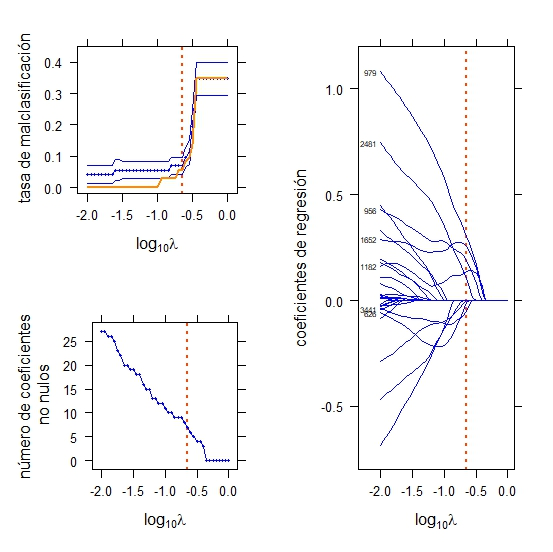
\includegraphics[width=0.9\textwidth]{leukemia_graficos}	\caption{ Elementos para la visualización de la regresión logística regularizada de los datos de leucemia}	
	\label{leukemia_graficos}
\end{figure}


A medida que el parámetro  $\lambda$ aumenta el tamaño de los coeficientes va dismi-\- nuyendo y se van anulando. 


El $\lambda$  óptimo seleccionado por validación cruzada con 20 es igual  a 0.028. Utilizando este valor para ajustar el modelo,  la tasa de mala clasificación  es pequeña, igual a  0.06.



\begin{table}
	\centering 
\begin{tabular}{cc|cc|c}
	\hline & & \multicolumn{3}{|c}{ Predichos } \\
	& & 0 & 1 & Total \\
	\hline Observados & 0 & 47 & 0 & 47 \\
  & 1 & 4 & 21 & 25 \\
	\cline { 2 - 5 } & Total & 51 & 21 & 72 \\
	\hline
\end{tabular}
\caption{Matriz de confusión }
\end{table}


%\begin{figure} [h]
%	\centering 
%	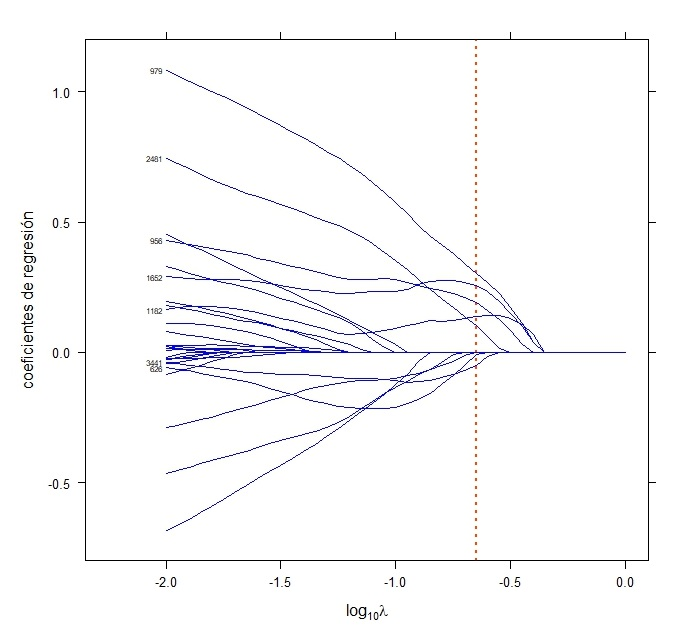
\includegraphics[width=0.8\textwidth]{leukemia_coef_reg}
%	\caption{ Coeficientes de regresión versus $\log(\lambda)$}
%	\label{leukemia_coef_reg }
%\end{figure}




%\begin{figure} [h]
%	\centering 
%	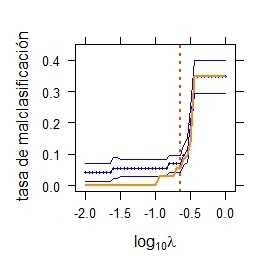
\includegraphics[width=0.8\textwidth]{leukemia_tasa_malclasif}
%	\caption{ Tasas de mal clasificación versus $\log(\lambda)$ }
%	\label{leukemia_tasa_malclasif}
%\end{figure}

 
 
 %\begin{figure} [h]
 %	\centering 
 %	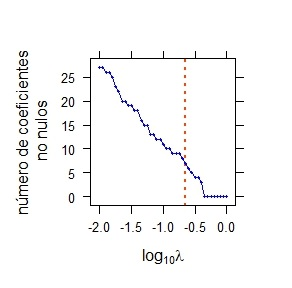
\includegraphics[width=0.8\textwidth]{ leukemia_coef_no_nulos}
 %	\caption{ Tasas de mal clasificación versus $\log(\lambda)$ }
 %	\label{ leukemia_coef_no_nulos}
 %\end{figure}
  
  
 
 
 %https://cran.r-project.org/web/packages/varbvs/vignettes/leukemia.html
 
 




\chapter{ Herramienta y desarrollo computacional }\label{herramienta}




Para abordar los problemas de clasificación multinomial explorados en esta tesis, se desarrolló una herramienta computacional en el lenguaje R. Esta herramienta permite realizar experimentos controlados que complementan el análisis teórico, brindando una perspectiva "práctica" sobre el desempeño de diferentes modelos de clasificación en escenarios simulados.





Para acceder al código fuente de la herramienta, se ha puesto a disposición un repositorio en GitHub que contiene todo el código necesario para ejecutar los experimentos. 
Se puede acceder al repositorio a través del siguiente link: \href{https://github.com/EAMolina500/Classifiers-Comparison}{\textcolor{blue}{\textit{Repositorio de GitHub}}}.

En la primera sección de este capítulo se describe la estructura del experimento de simulación que permitirá comparar el desempeño de los métodos de clasificación y en la segunda sección, la principal desde el punto de vista computacional, la descripción de la herramienta y el desarrollo computacional. 



\section{Estructura del experimento de simulación}


A continuación describimos los escenarios que utilizaremos para comparar los métodos de clasificación para estimar el modelo de regresión logístico multinomial definido. En lugar de utilizar la parametrización introducida en \eqref{logisticamult} (o su equivalente \eqref{logisticamultequiv}) usaremos la introducida por \cite{friedman2010}  


\begin{eqnarray*} 
	P(G=k \mid  \mathbf{X}=\mathbf{x})	&=&\frac{\text{e}^{  \beta_{k0}+\mathbf{x}^T\boldsymbol{\beta}_k  }}{\sum_{l=1}^{K} \text{e}^{  \beta_{l 0}+\mathbf{x}^T\boldsymbol{\beta}_{l}  }}, \; k=1\ldots, K 
\end{eqnarray*}

donde  $\mathbf{x} = (x_1,\ldots, x_p)^T$ y los coeficientes del modelo son $(\beta_{l0}, \boldsymbol{\beta}_{l}^T)$ con $\boldsymbol{\beta}_l^T = (\beta_{l1}, \ldots, \beta_{lp})$, $l = 1, \ldots, K$ y satisfacen las restricciones impuestas en \cite{zhu2004}.













\subsection*{Escenarios de simulación de los datos} 






\subsubsection*{Vector de características}

Asumiremos que el vector de variables características 

\begin{eqnarray}\label{modelocaract}
	\mathbf{X}^T=(X_1,\ldots, X_p)\sim N(\mathbf{0}, \Sigma).
\end{eqnarray}


Consideraremos dos tipos de estructuras para $\Sigma$: 


\begin{itemize}
	\item Modelo de variables características independientes (MI). $\Sigma=I$ es la matriz de identidad.
	% \item Modelo Autoregressive de orden 1, denotado por AR(1). Aquí, $\Sigma_{i j}=0.4^{|i-j|}$ for $i, j=1, \ldots p$ y $\boldsymbol{\Omega}=\Sigma^{-1}$.
	\item  Modelo con alta correlación (MAC). $\Sigma_{ij}=0\text{.}8$ si $i\neq j$, $i,j=1,\ldots, \left \lceil{p}\right \rceil /2$,    	 $\Sigma_{ii}=1$, $i=1,\ldots, p$ y $\Sigma_{ij}=0$ en las restantes entradas. Denotaremos esta matriz con $\Sigma_1$.  
\end{itemize}


\subsubsection*{Dimensión, tamaño muestral y número de clases}


Las dimensiones del vector $\mathbf{X}$ a considerar son $p=10, 50, 100$ y  $200$.  

Los números de clases son $K= 3,4,5,6,7$

Utilizaremos tamaños muestrales $n=1500$ para los datos de entrenamiento y $m=20000$ para los datos de prueba. Esto se aplicará tanto si $\Sigma$ satisface MI, como si satisface MAC, y para todos los números de clases mencionados.



\subsubsection*{Estructura de los vectores del modelo de regresión logística }



Los vectores del modelo de regresión logística son ralos, de tal modo que en el proceso de estimación un desafío es la   selección de variables.





\begin{itemize}
	\item Elegimos los coeficientes del modelo \eqref{logisticamultequiv} que satisfacen $\beta_{k0}=0$ y   una proporción 0.7 de las entradas de $\boldsymbol{\beta}_k$ son nulas.   Las entradas no nulas se generan con distribuciones uniformes en el intervalo [-0.5, 0.5]. 
	
	A modo de ejemplo, para $p=50$ con $K=3$ clases  $\boldsymbol{\beta}_1^T = (\beta_{11}, \ldots, \beta_{1p})$ tiene sus primeras 21 entradas iguales a cero y las restantes 9 generadas por una uniforme en el intervalo [-0.5, 0.5] y, $\boldsymbol{\beta}_2^T = (\beta_{21}, \ldots, \beta_{2p})$ tiene sus primeras 9 entradas generadas con una  uniforme en el mismo intervalo y las restantes entradas son nulas.  
\end{itemize}


Algunos de los métodos se rompen si no hay suficientes observaciones en las
clases, de allí que elegimos de  un modelo (casi) balanceado (con probabilidades
condicionales similares) y por ello también hemos elegido valores de  $n$ y $m$ grandes. 

La estimación de los valores esperados utilizan la noción de integración Monte Carlo introducida en la Sección 3.1 de \cite{casella2010}. 


Así, los datos de entrenamiento son generados del siguiente modo: 

\begin{itemize}
	\item Dado $K$ y $\Sigma$ generamos $\mathbf{x}_{i}^ {e}=(x_{i1}^{e},\ldots, x_{ip}^{e})^T$, $i=1,\ldots, n$ muestras independientes del vector \eqref{modelocaract}. 
	\item Computamos para cada $i$, la probabilidades condicionales $p_i=P(G=k|\mathbf{x}_i)$, $k=1,\ldots,  K$ utilizando  los coeficientes del modelo   $(\beta_{l0}, \boldsymbol{\beta}_{l}^T)$ con $\boldsymbol{\beta}_l^T = (\beta_{l1}, \ldots, \beta_{lp})$, $l = 1, \ldots, K-1$.
	Y, dado $i$, asignamos a $\mathbf{x}_i^{e}$ la clase cuya probabilidad condicional es máxima y la denotamos con $y_i^{e}$, $i=1,\ldots,n$. 
\end{itemize}

Análogamente generamos el conjunto de los $m$ datos test   $\mathbf{x}_j^{t}$ con su correspondiente clase  $y_j^{t}$, $j=1,\ldots,m$.

Este procedimiento se replica $R=50$ veces, obteniéndose $R$ conjuntos de datos de entrenamiento y de datos test.   

\subsubsection*{Métodos a comparar  }
Comparamos cinco métodos de clasificación lineal, utilizando bibliotecas de paquetes del lenguaje/entorno R descriptos a continuación. 
\begin{itemize}
	\item Análisis discriminante lineal (LDA). Usamos la función ``lda'' del paquete \texttt{MASS}. 
	\item Regresión logística multinomial (LM). La estimación del modelo usa la función ``multinom'' del paquete \texttt{nnet}. 
	\item Regresión logística multinomial con penalización lasso (LML). La función ``glmnet'' del paquete del mismo nombre estima el modelo logístico multinomial utilizando como argumentos family = multinomial y alpha=1. La penalización óptima se halla por validación cruzada. 
	\item Bosques aleatorios (RF) utiliza la función randomForest de la librería \texttt{randomForest}, del paquete del mismo nombre. 
	\item Regresión logística multinomial con penalización red elástica (LME). Análoga a LML  pero $\alpha=1/2$. 
\end{itemize}



\subsubsection*{Medidas de desempeño}

Para este breve informe sólo elegimos la tasa de mala clasificación  o de clasificación incorrecta, $M_R$.  La tasa de error test es desconocida, de allí que nosotros la estimaremos, con lo cual deberíamos escribir $\widehat{M}_R$ pero para simplificar la notación eliminamos el ``sombrero''.

Si $\delta^{e}$ es un clasificador entrenado con los datos de entrenamiento, para una réplica $r$ consideramos $\widehat{y}_j$ la clase predicha por  $\delta^{e}$ para cada observación $\mathbf{x}_j^{t}$, $j=1,\ldots,m$.  La tasa de mala clasificación  para la $r$-ésima réplica se define como:

\begin{eqnarray}\label{tasaentremuestr}
	M_R^{(r)}=\frac 1m \# \left\{  {j\in \{1,\ldots,m \}: y_j^{t}\neq \widehat{y}_j }	\right\},\; r=1,\ldots, R
\end{eqnarray}

Es importante tener en cuenta que estamos estimando la tasa de error test, discutida en la Sección 2.2.3 de \citep{james2021}. 


Para medir el desempeño de la selección de variables - identificación correcta de los coeficientes nulos- utilizamos las medidas ``precision'' y ``recall'', precisión y exahustividad en castellano,   que serán denotados con $\mathrm{PR}$ y $\mathrm{RC}$.  Las medidas se definen,  para la $r$-ésima réplica, como:


$$
\mathrm{RC}^{(r)}=\frac{\sum_{j=1}^p \text{I}\left(\beta_j \neq 0, \hat{\beta}_j^{(r)} \neq 0\right)}{\sum_{j=1}^p  \text{I}\left(\beta_j \neq 0\right)}, \quad \mathrm{PR}^{(r)}=\frac{\sum_{j=1}^p \text{I}\left(\beta_j \neq 0, \hat{\beta}_j^{(r)} \neq 0\right)}{\sum_{j=1}^p \text{I}\left(\hat{\beta}_j^{(r)} \neq 0\right)}
$$
donde, $r=1\ldots R$, I es una variable indicadora,  $\boldsymbol{\beta}_0=\left(\beta_1, \ldots, \beta_p\right)^T$ y  $\hat{\boldsymbol{\beta}}^{(r)}=\left(\hat{\beta}_1, \ldots, \hat{\beta}_p\right)^T $ son los coeficientes verdaderos y  estimados, respectivamente.


Así, $\sum_{j=1}^p \text{I}\left(\beta_j \neq 0, \hat{\beta}_j \neq 0\right)$ cuenta el número de coeficientes $\beta_j$  que son no nulos y tal que su estimador $\hat{\beta}_j$ es también diferente de cero,  $\sum_{j=1}^p  \text{I}\left(\beta_j \neq 0\right)$ y $\sum_{j=1}^p  \text{I}\left(\beta_j \neq 0\right)$ cuentan el número de coeficientes del modelo  y estimados no nulos respectivamente.


De este modo $\mathrm{RC}$ mide la proporción de variables que participan del modelo $\left(\beta_j \neq 0\right)$ y que la estimación logra identificar correctamente ( $\hat{\beta}_j \neq 0$ ), en relación al total de coeficientes verdaderos no nulos.  Y de modo análogo  $\mathrm{PR}$ mide esa proporción pero respecto de los coeficientes estimados  no nulos. Ambas medidas asumen valores en el intervalo $[0,1]$.  El desempeño de un método de estimación es mejor cuanto las medias de $ \mathrm{RC}$ y $ \mathrm{PR}$ se acerquen a 1. 

Las medidas  $ \mathrm{RC}$ y $ \mathrm{PR}$  sólo las computaremos para LML y LME dado que ya sabemos que LM no selecciona variables y los restantes métodos no estiman el modelo de regresión logístico. 

Como medidas de resumen   computamos la media y el desvío estándar de la muestras  $M_R^{(r)}$, $ \mathrm{RC}^{(r)}$ y $ \mathrm{PR}^{(r)}$  $r=1\ldots, R$. 








\section{Desarrollo computacional }\label{herramientadesarrollos}
\subsection*{Lenguaje de Programación:} 

Se utilizó el lenguaje R debido a su robustez y versatilidad en el ámbito de la estadística y el aprendizaje automático. R proporciona un amplio ecosistema de paquetes para la generación de datos simulados, el ajuste de modelos estadísticos y el análisis de resultados.

\subsection*{Propósito:}

Se desarrolló una herramienta computacional escalable, diseñada para realizar experimentos controlados en la comparación de modelos de clasificación multinomial en el contexto de problemas de clasificación. 

\subsection*{Funcionamiento:}

A través de simulaciones, permite generar datos, entrenar diversos modelos, realizar predicciones y evaluar métricas clave como la tasa de error de clasificación, precisión y recall. 

Esta herramienta está orientada a brindar una aproximación experimental complementaria al análisis matemático teórico presentado en la tesis, explorando cómo los métodos de clasificación funcionan en situaciones controladas. También, ofreciendo una plataforma que puede extenderse para abordar otros métodos de clasificación o escenarios de simulación.

\subsection*{Librerías:}

El script principal de este trabajo emplea varias librerías que facilitan tareas específicas:

\begin{itemize}
	\item \texttt{Matrix}: para manipulación de matrices dispersas.
	
	\item \texttt{MASS}: para métodos estadísticos y generación de datos mediante distribuciones normales multivariadas.
	
	\item \texttt{randomForest}: para el ajuste de modelos Random Forest.
	
	\item \texttt{glmnet}: para regresión penalizada (Lasso y Elastic Net).
	
	\item \texttt{mvnfast}: para generación eficiente de datos multivariados.
	
	\item \texttt{nnet}: para regresión logística multinomial.
\end{itemize}

\subsection*{Estructura del Script:} 

El mismo está organizado en módulos funcionales. Incluye algunas funciones importantes descriptas abajo, y otras funciones "auxiliares" para complementar a las primeras y mantener la claridad del código. 

\begin{itemize}
\item Función "Simulate":  

La función Simulate es el núcleo de la herramienta, gestionando múltiples réplicas de simulaciones y recopilando los resultados. Permite explorar el desempeño de diversos métodos de clasificación y regresión en escenarios repetidos y controlados, variando parámetros clave como tamaño de muestra, número de clases y correlación entre variables.

\item Función "Train":
 
La función Train encapsula la lógica para entrenar varios modelos de aprendizaje supervisado, incluidos Análisis Discriminante Lineal (LDA), Regresión Logística, Lasso, Elastic Net y Random Forest. Proporciona una interfaz unificada para ajustar modelos a diferentes conjuntos de datos simulados o reales.

\item Función "Predict":  

La función Predict se utiliza para realizar predicciones a partir de los modelos entrenados. Adapta su comportamiento según el método utilizado, como predicción basada en regularización (usando `lambda.min` en modelos como Lasso y Elastic Net) o predicción estándar en métodos como LDA o Random Forest.

\item Función "CalculatePrecisionAndRecall":  

Esta función calcula las métricas de precisión y recall para evaluar la capacidad de los modelos basados en regularización al identificar correctamente las variables relevantes. Utiliza los coeficientes estimados ($beta.hat$) y los coeficientes reales ($beta.list$) para generar estas métricas.

\item Función "GetLambdaMinByCrossValidation":  

La función encuentra el valor óptimo de penalización (`lambda.min`) para modelos de regularización como Lasso o Elastic Net mediante validación cruzada. Este valor se utiliza para ajustar el modelo con el mejor balance entre ajuste y simplicidad.

\item Funciones para la generación de datos:  

Estas funciones generan datos simulados para experimentos, utilizando distribuciones multivariadas normales ($mvrnorm$) configuradas con una matriz de covarianza ($sigma$) y coeficientes ($beta.list$). Esto permite crear escenarios controlados con diferentes niveles de complejidad y correlación entre variables.

\item Funciones para la preparación de datos: 

Estas funciones transforman y organizan los datos generados en formatos adecuados para el entrenamiento y evaluación de modelos. Incluyen la asignación de etiquetas, normalización de características y división en conjuntos de entrenamiento y prueba.

\item Funciones para la evaluación de modelos:  

La función Evaluate mide la tasa de error de clasificación como la proporción de etiquetas predichas incorrectamente. Es una métrica clave para comparar el desempeño de diferentes modelos y analizar su precisión bajo diversos escenarios.

\item Funciones para el cálculo de métricas:

Estas funciones están diseñadas para calcular errores y métricas específicas dependiendo del método empleado. Por ejemplo, evalúan la tasa de error de clasificación, la precisión y/o el recall, adaptándose a las características de cada modelo. 

\item Funciones de soporte:

Estas funciones incluyen tareas como la preparación de datos, extracción de coeficientes y manejo de resultados intermedios, optimizando el flujo de trabajo al estructurar datos de entrada y salida y facilitando la interpretación y visualización de los resultados, así como la integración con otros módulos.

\end{itemize}


\subsection*{Buenas prácticas:}

\begin{itemize}
	\item Modularidad: Cada tarea (por ejemplo, entrenamiento, predicción, evaluación y cálculo de métricas) está implementada en funciones independientes para maximizar la claridad, la reusabilidad y la adaptabilidad del código.
	
	\item Gestión de errores: Se utilizan bloques \texttt{tryCatch} para capturar y manejar errores durante el entrenamiento, predicción y cálculo de métricas, evitando interrupciones en los procesos y registrando fallas para diagnóstico posterior.
	
	\item Flexibilidad: Las funciones \texttt{Train} y \texttt{Predict} están diseñadas para permitir la integración de nuevos métodos de clasificación con facilidad. Esto se logra mediante el uso de estructuras condicionales (como \texttt{switch}) y parámetros modulares que aseguran una expansión controlada.
	
	\item Uso eficiente de recursos: La validación cruzada, las simulaciones y el cálculo de métricas están diseñados para minimizar cómputos redundantes. Por ejemplo, valores como \texttt{lambda.min} se calculan una sola vez y se reutilizan de manera eficiente en diferentes partes del flujo.
	
	\item Rendimiento computacional: Se implementan prácticas para optimizar el tiempo de ejecución, como el procesamiento por bloques (estructuras \texttt{for} controladas) y el registro detallado del tiempo total de simulación y evaluación para identificar cuellos de botella.
	
	\item Documentación: El código incluye comentarios y explicaciones detalladas que describen la funcionalidad de cada sección. Esto, junto con nombres consistentes y autoexplicativos para las funciones, parámetros y variables, facilita la interpretación, el mantenimiento y la colaboración.

	\item Pruebas y validación: El diseño incluye pruebas internas de las funciones clave, verificando la consistencia de los resultados y asegurando que se comporten como se espera en una amplia gama de escenarios.

	\item Organización futura del código: Cabe destacar que, por simplicidad, el código se ha mantenido en un solo archivo. Sin embargo, para facilitar su mantenimiento y escalabilidad en el futuro, sería recomendable dividirlo en múltiples archivos. Esto permitiría organizar las funciones de manera más eficiente, agrupando aquellas relacionadas entre sí (por ejemplo, funciones de entrenamiento y predicción en un archivo, generación de datos en otro), lo que mejoraría la legibilidad y facilitaría la incorporación de nuevas funcionalidades o mejoras.
	
	\item Convenciones de escritura de código: Se han seguido convenciones de escritura de código para garantizar la coherencia y legibilidad en todo el proyecto. Estas convenciones incluyen normas para la nomenclatura de funciones y variables, la estructura del código, y la indentación. Para más detalles sobre las convenciones utilizadas, se puede consultar el siguiente link: \href{https://www.datanalytics.com/2014/01/27/guia-de-estilo-de-r-de-google/}{\textcolor{blue}{\textit{Guía de estilo de R}}}.


\end{itemize}






  \chapter{ Ensayos y resultados}\label{reglogmult}
  
  
  
  
   A continuación mostramos y discutimos los resultados del experimento de simulación descripto en la Sección 4.1 para el modelo regresión logística multinomial. 
  
  Recordamos que el objetivo de este experimento es evaluar el comportamiento de los métodos de estimación del modelo de regresión logística multinomial. El modelo fue definido en \eqref{logisticamult} (o su equivalente \eqref{logisticamultequiv}) y como se mencionó, para la simulación se utiliza la parametrización introducida por \cite{friedman2010}.  
  
  
  
  
  
 
 
  
 
 Para el modelo de variables independientes, con matriz de covarianza igual a la identidad, las Tablas \ref{tablak3sigmaiden}, \ref{tablak4sigmaiden}, \ref{tablak5sigmaiden}, \ref{tablak6sigmaiden} y   \ref{tablak7sigmaiden} del Apéndice B muestran las medias y desvíos de las tasas de $M_R$ y las Tablas \ref{tablak3sigmaidenpr}, \ref{tablak4sigmaidenpr}, \ref{tablak5sigmaidenpr}, \ref{tablak6sigmaidenpr} y   \ref{tablak7sigmaidenpr} las medias de $ \mathrm{RC}$  y $ \mathrm{PR}$ para $K=3, 4, 5,6 $ y $7$  respectivamente.   Análogamente, las Tablas 	\ref{tablak3corralta} a \ref{tablak7corraltapr} para el modelo  de alta correlación.  
 
 
 Las Figuras  \ref{boxk3sigmaiden} a  \ref{boxk7sigmaiden} comparan los diagramas de caja 
para los valores de   $M_R$ en el modelo con $\Sigma=I$, mientras que  las Figuras  \ref{boxk3alta} a  \ref{boxk7alta} lo hacen para el modelo de alta correlación con $\Sigma=\Sigma_1$.


 
 Algunas conclusiones preliminares son las siguientes:
 
 \begin{itemize}
 	\item  Para $K$ fijo, las medias de las tasas de mala clasificación  aumentan cuando el número de variables $p$ crece, mostrando que la dificultad de estimación es mayor. Y para $p$ fijo, dichas medias aumentan cuando $K$ crece, aunque hay que tener en cuenta el efecto de los tamaños $n$ y $m$. Este fenómeno ocurre en ambos modelos MI y MAC.
 	\item En general las medias de RC asumen valores altos y en cambio las de PR son bajos. Esto implica que los métodos de regularización identifican los coeficientes no nulos ( RC alto) pero producen coeficientes estimados no nulos cuando los correspondientes coeficientes del modelo son ceros.
 	
 	\item  LDA y RF tienen el peor desempeño comparados con los métodos que regularizan (LML y LME). Para  casi todas las situaciones LML tiene mejor desempeño, de acuerdo al comportamiento de $M_R$, que LME.   Y comparativamente de acuerdo a RC y PR, también LME se desempeña un poco mejor que LML.
 	
 	   
 	
 \end{itemize}
 
 
 
 
 
 
 
 
 
 \section{ Análisis de datos de genómica }
 
 
 En Vincent y Hansen (2014) se mencionan  ejemplos de bases de datos reales, entre ellas la correspondiente a la localización de ciertos tipos de cáncer, que se halla en el repositorio público de datos de genómica funcional GEO (ver  \href{https://healthdata.gov/dataset/Gene-Expression-Omnibus-GEO-/ypwa-g5v3/about_data}{Geo}). El conjunto de datos consiste de  expresiones génicas- microARNs- obtenidas por la técnica ``bead-based'' provenientes de  muestras de tejidos normales y cancerosos.  Aquí la palabra muestra alude a una observación y la expresión génica se refiere a una variable característica o explicatoria.  
 
 En el sitio  \href{https://github.com/nielsrhansen/msgl/blob/master/data/PrimaryCancers.RData}{Hansen} correspondiente a uno de los autores del trabajo mencionado se puede acceder a un subconjunto de la base de datos, que cuenta con 165 pacientes (filas de la matriz de datos), 371 variables o expresiones génicas (columnas de la matriz de datos)  y la variable categórica respuesta $Y$ que denota localización o tipo de cáncer con las siguientes 8 clases: 
 \begin{itemize}
 	\item Cáncer de mama, abreviado con ``Breast''.
 	\item Colangiocarcinoma abreviado como ``CCA'' %(ver  \href{https://cancerquest.org/es/para-los-pacientes/cancer-por-tipo/colangiocarcinoma}{CQ})
 	\item  Cirrosis abreviado como `` Cirrhosis''.
 	\item Cáncer de la unión esófago gástrico,   denotado con ``EG''.
 	\item Carcinoma hepatocelular, abreviado con ``HCC''.
 	\item Cáncer de Hígado, abreviado como  ``Liver''. 
 	\item 						Cáncer de Páncreas, denotado con ``Pancreas''.
 	\item Carcinoma de células escamosas, abreviado con ``Squamous''.
 	
 \end{itemize}
 
 Así la matriz de los datos tiene dimensión $165\times (371+1)$, y en la última columna alojamos a la variable respuesta $Y$.
 
 
 En la Tabla 	\ref{cancer} se pueden observar las frecuencias absolutas para las localizaciones. 
 
 
 \begin{table}[h]
 	\mbox{}\hfill
 	
 	\centering{ 
 		
 		\scalebox{0.75}{
 			\begin{tabular}{l|r }
 				
 				\hline
 				
 				Localización &Frecuencia \\
 				
 				\hline
 				
 				Breast  &   17                \\
 				
 				CCA  &   20                \\
 				Cirrhosis  &   17                \\
 				CRC  &   20                \\
 				EG  &   18                \\
 				HCC  &   17                \\
 				Liver  &   20                \\
 				Pancreas &   20                \\
 				
 				Squamous &   16  \\
 				
 				
 				\hline
 				
 		\end{tabular}}
 		
 	}
 	
 	\caption{  Frecuencias absolutas de las clases de localizaciones del  cáncer} 
 	\label{cancer}
 	
 \end{table} 
 
 
 En la Tabla \ref{desempmetodoscancer} se muestran las medias y desvíos de las tasas de mala clasificación  para los métodos estudiados en la sección de simulación. Para cada réplica se eligen al azar 130 filas de la base de datos como datos de entrenamiento y las restantes filas como datos test. El procedimiento es costoso computacionalmente de allí que se replica 10 veces. 
 
 Notar que el algoritmo logística multinomial (LG) tiene el peor desempeño, bosques aleatorios y análisis discriminante lineal se comportan parecido y el que posee la menor tasa de mala clasificación  es el método logística multinomial con penalización red elástica (LME).
 
 
 
 \begin{table}[h]
 	\mbox{}\hfill
 	
 	\centering{ 
 		
 		\scalebox{0.75}{
 			\begin{tabular}{l|r }
 				
 				\hline
 				
 				Métodos & $M_R$  \\
 				
 				\hline
 				
 				LDA  &  0.309          \\
 				
 				& (0.055)        \\
 				
 				
 				LG & 0.546       \\
 				
 				
 				
 				& (0.052)         \\
 				
 				
 				
 				LML &   0.312    \\
 				
 				
 				
 				& (0.038)       \\
 				
 				
 				
 				RF &  0.309      \\
 				
 				
 				
 				& (0.032)        \\
 				
 				
 				
 				LME  & {\bf 0.282}     \\
 				
 				
 				
 				& (0.038)     \\
 				
 				
 				
 				
 				\hline
 				
 		\end{tabular}}
 		
 	}
 	
 	\caption{ Media y desvío estándar (entre paréntesis) de $M_R^{(r)}$, $r=1,\ldots, 10$.   } 
 	\label{desempmetodoscancer}
 	
 \end{table} 
 
 
 
 \begin{figure} [h]
 	\centering 
 	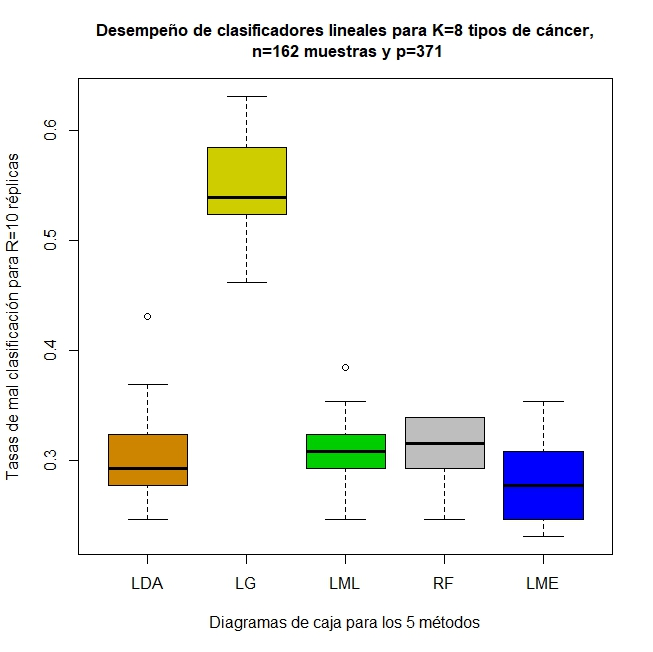
\includegraphics[width=0.5\textwidth]{boxplot_cancer_p130_R10}
 	\caption{ Diagramas de caja para la tasa de mala clasificación  a lo largo de $R=10$ réplicas para la base de datos de localizaciones de cáncer.}
 	\label{boxplot_cancer_p130_R10}
 \end{figure}
 
 \newpage
 


  \chapter{Conclusiones y trabajos futuros}\label{conclus}
  
 En este trabajo, se evaluaron  métodos de clasificación, antes mencionados, aplicados a problemas multiclase con tres clases o más. Los resultados indican que, a medida que aumenta la cantidad de variables, el desempeño de los clasificadores tiende a deteriorarse.

 Cuando el modelo es ralo (es decir, solo unas pocas variables explicativas son realmente importantes para la clasificación), los métodos que aplican regularización, como la regresión logística lasso y la red elástica, muestran una ventaja notable.
Estos métodos penalizan las variables menos importantes, favoreciendo soluciones más parsimoniosas, y reduciendo así el riesgo de sobre-ajuste. Al mismo tiempo este hecho  mejora la estimación del modelo permitiendo que se desempeñe mejor con datos desconocidos- disminuyendo la tasa de error test, y aumentando su utilidad práctica en problemas multiclase complejos. 


 A partir del análisis realizado, también podemos destacar la importancia de las técnicas de remuestreo para estimar de manera robusta el error de clasificación y, a su vez, comparar objetivamente el desempeño entre distintos clasificadores. Este enfoque es especialmente útil cuando se dispone de conjuntos de datos limitados, ya que facilita una evaluación confiable del modelo sin necesidad de grandes muestras de validación. 

 Finalmente, para problemas en los que el número de clases es particularmente alto, este estudio sugiere la exploración de técnicas de fusión de clases. La fusión de clases es un estrategia prometedora que podría simplificar la estructura del problema, agrupando categorías similares para reducir la complejidad del modelo. Esto no solo facilitaría la interpretación de los resultados, sino que también puede mejorar la precisión de los métodos de clasificación al reducir el espacio de decisión.

 En conclusión, este estudio contribuye a una comprensión más profunda de los factores que afectan el rendimiento de los clasificadores multiclase y proporciona recomendaciones prácticas sobre el uso de métodos de regularización y técnicas de remuestreo en modelos ralos. Estos hallazgos son de particular interés para aquellos que enfrentan problemas de clasificación multiclase en entornos con alta dimensionalidad y limitaciones de datos, y sugieren nuevas direcciones para mejorar la eficiencia y efectividad de los métodos de clasificación en escenarios complejos.
  
  
   \section*{Apéndice A. Notas sobre la regresión logística multinomial}\label{apenreglog}
  
  
  
  
  En esta sección  extendemos el algoritmo introducido en la Sección \ref{estimamrlmulti} al caso $K>2$, basados en \cite{htf} y en las Notas  \href{https://yuhangzhou88.github.io/ESL_Solution/ESL-Solution/4-Linear-Methods-for-Classification/ex4-4/}{Zhou}). 
  
  
  Como antes, sea 
  $$
  P(G=k \mid X=x)=\frac{\text{e}^{\boldsymbol{\beta}_k^T x }}{1+\sum_{l=1}^{K-1} \text{e}^{\boldsymbol{\beta}_l^T x }  }, k=1, \ldots, K-1
  $$
  y
  $$
  P(G=K \mid X=x)=\frac{1}{1+\sum_{l=1}^{K-1} \text{e}^{\boldsymbol{\beta}_l^T x }}.
  $$
  Cada  $ \boldsymbol{\beta}_k \in \mathbb{R}^{p+1}$ para $k=1, \ldots, K-1$. Denotemos $ \boldsymbol{\beta}^T=\left ( \boldsymbol{\beta}_1^T, \ldots,  \boldsymbol{\beta}_{K-1}^T\right)$ tal que  $ \boldsymbol{\beta}$, el cual tiene dimensión $(p+1)(K-1)$. 
  
  Sea 
  $$
  p_k(x ;  \boldsymbol{\beta})=P(G=k \mid X=x) .
  $$
  
  La función de log-verosimilitud es 
  $$
  l( \boldsymbol{\beta})=\sum_{i=1}^n \log p_{g_i}\left(\mathbf{x}_i ;  \boldsymbol{\beta}\right)
  $$
  
  Como antes, codificamos las clases de 1 a $K$, y utilizamos indicadoras; así 
  $$
  \begin{aligned}
  	l( \boldsymbol{\beta}) & =\sum_{i=1}^n\left(\sum_{k=1}^{K-1} \mathbf{1}\left(y_i=k\right) \log p_k\left(\mathbf{x}_i ;  \boldsymbol{ \boldsymbol{\beta}}\right)-\mathbf{1}\left(y_i=K\right) \log \left(1+\sum_{l=1}^{K-1} \text{e}^{ \boldsymbol{\beta}_l^T} x_l\right)\right) \\
  	& =\sum_{i=1}^n\left(\sum_{k=1}^{K-1} \mathbf{1}\left(y_i=k\right)  \boldsymbol{\beta}_k^T \mathbf{x}_i-\log \left(1+\sum_{l=1}^{K-1} \text{e}^{ \boldsymbol{\beta}_l^T x_l}\right)\right).
  \end{aligned}
  $$
  Para maximizar $	l( \boldsymbol{\beta})$ derivamos e igualamos a cero y obtenemos las ecuaciones score. Así,  para $k=1, \ldots, K-1$, $	\dst \frac{\partial l( \boldsymbol{\beta})}{\partial  \boldsymbol{\beta}_k} \in \mathbb{R}^{p+1}$ puede ser escrita como
  
  
  \begin{eqnarray}\label{derivpri}
  	\frac{\partial l( \boldsymbol{\beta})}{\partial  \boldsymbol{\beta}_k} & =&\sum_{i=1}^n\left(\mathbf{1}\left(y_i=k\right) \mathbf{x}_i-\frac{\mathbf{x}_i \text{e}^{ \boldsymbol{\beta}_k^T \mathbf{x}_i}}{1+\sum_{l=1}^{K-1} \text{e}^{ \boldsymbol{\beta}_l^T x_l}}\right) \nonumber \\
  	& =& \sum_{i=1}^n \mathbf{x}_i\left(\mathbf{1}\left(y_i=k\right)-\frac{\text{e}^{ \boldsymbol{\beta}_k^T \mathbf{x}_i}}{1+\sum_{l=1}^{K-1} \text{e}^{ \boldsymbol{\beta}_l^T x_l}}\right) 
  \end{eqnarray}
  
  
  Escribamos 
  $$
  \frac{\partial l( \boldsymbol{\beta})}{\partial  \boldsymbol{\beta}}=\left(\begin{array}{c}
  	\frac{\partial l( \boldsymbol{\beta})}{\partial  \boldsymbol{\beta}_1} \\
  	\vdots \\
  	\frac{\partial l( \boldsymbol{\beta})}{\partial  \boldsymbol{\beta}_{K-1}}
  \end{array}\right) \in \mathbb{R}^{(p+1)(K-1)} .
  $$
  
  
  Para las derivadas de orden 2, observemos que para $k \neq j \in\{1, \ldots, K-1\}$, obtenemos:
  \begin{eqnarray}\label{orden2kj}
  	\frac{\partial^2 l( \boldsymbol{\beta})}{\partial  \boldsymbol{\beta}_k \partial  \boldsymbol{\beta}_j^T} & =&\sum_{i=1}^n \mathbf{x}_i\left(-\frac{\text{e}^{ \boldsymbol{\beta}_j^T \mathbf{x}_i} \mathbf{x}_i^T \text{e}^{ \boldsymbol{\beta}_k^T \mathbf{x}_i}}{\left(1+\sum_{l=1}^{K-1} \text{e}^{ \boldsymbol{\beta}_l^T \mathbf{x}_i}\right)^2}\right)\nonumber  \\
  	& =& -\sum_{i=1}^n \mathbf{x}_i \mathbf{x}_i^T \frac{\text{e}^{ \boldsymbol{\beta}_k^T \mathbf{x}_i}}{1+\sum_{l=1}^{K-1} \text{e}^{ \boldsymbol{\beta}_l^T \mathbf{x}_i}} \cdot \frac{\text{e}^{ \boldsymbol{\beta}_j^T \mathbf{x}_i}}{1+\sum_{l=1}^{K-1} \text{e}^{ \boldsymbol{\beta}_l^T \mathbf{x}_i}} \nonumber \\
  	& =& -\sum_{i=1}^n \mathbf{x}_i \mathbf{x}_i^T p_k\left(\mathbf{x}_i ;  \boldsymbol{\beta}\right) p_j\left(\mathbf{x}_i ;  \boldsymbol{\beta}\right) .
  \end{eqnarray}
  
  
  Para $k \in\{1, \ldots, K-1\}$, obtenemos
  \begin{eqnarray}\label{orden2kk}
  	\frac{\partial^2 l( \boldsymbol{\beta})}{\partial  \boldsymbol{\beta}_k \partial  \boldsymbol{\beta}_k^T} & =&\sum_{i=1}^n \mathbf{x}_i\left(-\frac{\text{e}^{ \boldsymbol{\beta}_k^T} \mathbf{x}_i^T}{\left(1+\sum_{l=1}^{K-1} \text{e}^{ \boldsymbol{\beta}_l^T \mathbf{x}_i}\right)^2}\right)\nonumber  \\
  	& =&-\sum_{i=1}^n \mathbf{x}_i \mathbf{x}_i^T \frac{\text{e}^{ \boldsymbol{\beta}_k^T}}{1+\sum_{l=1}^{K-1} \text{e}^{ \boldsymbol{\beta}_l^T \mathbf{x}_i}} \cdot \frac{1}{1+\sum_{l=1}^{K-1} \text{e}^{ \boldsymbol{\beta}_l^T \mathbf{x}_i}} \nonumber  \\
  	& =&-\sum_{i=1}^n \mathbf{x}_i \mathbf{x}_i^T p_k\left(\mathbf{x}_i ;  \boldsymbol{\beta}\right) p_k^c\left(\mathbf{x}_i ;  \boldsymbol{\beta}\right)
  \end{eqnarray}
  donde  $p_k^c\left(\mathbf{x}_i ;  \boldsymbol{\beta}\right)=1-p_k\left(\mathbf{x}_i ;  \boldsymbol{\beta}\right)$.
  
  
  De modo compacto podemos escribir 
  $$
  \frac{\partial^2 l( \boldsymbol{\beta})}{\partial  \boldsymbol{\beta} \partial  \boldsymbol{\beta}^T}=\left(\begin{array}{cccc}
  	\frac{\partial^2 l( \boldsymbol{\beta})}{\partial  \boldsymbol{\beta}_1 \partial  \boldsymbol{\beta}_1^T} & \frac{\partial^2 l( \boldsymbol{\beta})}{\partial  \boldsymbol{\beta}_1 \partial  \boldsymbol{\beta}_2^T} & \cdots & \frac{\partial^2 l( \boldsymbol{\beta})}{\partial  \boldsymbol{\beta}_1 \partial  \boldsymbol{\beta}_{K-1}^T} \\
  	\frac{\partial^2 l( \boldsymbol{\beta})}{\partial  \boldsymbol{\beta}_2 \partial  \boldsymbol{\beta}_2^T} & \frac{\partial^2 l( \boldsymbol{\beta})}{\partial  \boldsymbol{\beta}_2 \partial  \boldsymbol{\beta}_2^T} & \cdots & \frac{\partial^2 l( \boldsymbol{\beta})}{\partial  \boldsymbol{\beta}_2 \partial  \boldsymbol{\beta}_{K-1}^T} \\
  	\vdots & \vdots & \ddots & \vdots \\
  	\frac{\partial^2 l( \boldsymbol{\beta})}{\partial  \boldsymbol{\beta}_{K-1} \partial  \boldsymbol{\beta}_1^T} & \frac{\partial^2 l( \boldsymbol{\beta})}{\partial  \boldsymbol{\beta}_{K-1} \partial  \boldsymbol{\beta}_2^T} & \cdots & \frac{\partial^2 l( \boldsymbol{\beta})}{\partial  \boldsymbol{\beta}_{K-1} \partial  \boldsymbol{\beta}_{K-1}^T}
  \end{array}\right) \in \mathbb{R}^{(K-1)(p+1) \times(K-1)(p+1)}
  $$
  
  
  Comenzando con $ \boldsymbol{\beta}^{\text {viejo }}$, una actualización del algoritmo de Newton viene dada por:
  $$
  \boldsymbol{\beta}^{\text {nuevo }}= \boldsymbol{\beta}^{\text {viejo }}-\left(\frac{\partial^2 l( \boldsymbol{\beta})}{\partial  \boldsymbol{\beta} \partial  \boldsymbol{\beta}^T}\right)^{-1} \frac{\partial l( \boldsymbol{\beta})}{\partial  \boldsymbol{\beta}}
  $$
  donde las derivadas  son evaluadas en $ \boldsymbol{\beta}^{\text {viejo }}$. 
  
  
  Alcancemos una escritura más compacta en forma matricial. Primero denotemos, para $k=1, \ldots, K-1$,
  $$
  \mathbf{y}_k=\left(\begin{array}{c}
  	\mathbf{1}\left(y_1=k\right) \\
  	\mathbf{1}\left(y_2=k\right) \\
  	\vdots \\
  	\mathbf{1}\left(y_n=k\right)
  \end{array}\right), \mathbf{X}=\left(\begin{array}{c}
  	x_1^T \\
  	x_2^T \\
  	\vdots \\
  	x_n^T
  \end{array}\right), \quad \mathbf{p}_k=\left(\begin{array}{c}
  	p_k\left(x_1 ;  \boldsymbol{\beta}\right) \\
  	p_k\left(x_2 ;  \boldsymbol{\beta}\right) \\
  	\vdots \\
  	p_k\left(x_n ;  \boldsymbol{\beta}\right)
  \end{array}\right)
  $$
  
  
  Entonces  \eqref{derivpri} se puede expresar  
  $$
  \frac{\partial l( \boldsymbol{\beta})}{\partial  \boldsymbol{\beta}_k}=\mathbf{X}^T\left(\mathbf{y}_k-\mathbf{p}_k\right)
  $$
  
  
  Si ahora definimos 
  $$
  \mathbf{y}=\left(\begin{array}{c}
  	\mathbf{y}_1 \\
  	\mathbf{y}_2 \\
  	\vdots \\
  	\mathbf{y}_{K-1}
  \end{array}\right) \text { and } \mathbf{p}=\left(\begin{array}{c}
  	\mathbf{p}_1 \\
  	\mathbf{p}_2 \\
  	\vdots \\
  	\mathbf{p}_{K-1}
  \end{array}\right)
  $$
  podemos escribir:
  \begin{eqnarray}\label{Xhat}
  	\frac{\partial l( \boldsymbol{\beta})}{\partial  \boldsymbol{\beta}}=\left(\begin{array}{cccc}
  		\mathbf{X}^T & 0 & \cdots & 0 \\
  		0 & \mathbf{X}^T & \cdots & 0 \\
  		\vdots & \vdots & \ddots & \vdots \\
  		0 & 0 & \cdots & \mathbf{X}^T
  	\end{array}\right)\left(\begin{array}{c}
  		\mathbf{y}_1-\mathbf{p}_1 \\
  		\mathbf{y}_2-\mathbf{p}_2 \\
  		\vdots \\
  		\mathbf{y}_{K-1}-\mathbf{p}_{K-1}
  	\end{array}\right)=\hat{\boldsymbol{X}}(\mathbf{y}-\mathbf{p})
  \end{eqnarray}
  
  
  donde  $\hat{\boldsymbol{X}}$ es la matriz de arriba con $\mathbf{X}^T$ sobre las posiciones de la diagonal.
  
  
  Para $k=1, \ldots, K-1$, sea
  $$
  \mathbf{P}_k=\left(\begin{array}{cccc}
  	p_k\left(x_1 ;  \boldsymbol{\beta}\right) p_k^c\left(x_1 ;  \boldsymbol{\beta}\right) & 0 & \cdots & 0 \\
  	0 & p_k\left(x_2 ;  \boldsymbol{\beta}\right) p_k^c\left(x_2  \boldsymbol{\beta}\right) & \cdots & 0 \\
  	\vdots & \vdots & \ddots & \vdots \\
  	0 & 0 & \cdots & p_k\left(x_n ;  \boldsymbol{\beta}\right) p_k^c\left(x_n ;  \boldsymbol{\beta}\right)
  \end{array}\right)
  $$
  
  
  Utilizando \ref{orden2kk},  tenemos  para $k=1, \ldots, K-1$ que
  $$
  \frac{\partial^2 l( \boldsymbol{\beta})}{\partial  \boldsymbol{\beta}_k \partial  \boldsymbol{\beta}_k^T}=-\mathbf{X}^T \mathbf{P}_k \mathbf{X}
  $$
  Para $k=1, \ldots, K-1$, consideremos
  $$
  \mathbf{R}_k=\left(\begin{array}{cccc}
  	p_k\left(x_1 ;  \boldsymbol{\beta}\right) & 0 & \cdots & 0 \\
  	0 & p_k\left(x_2 ;  \boldsymbol{\beta}\right) & \cdots & 0 \\
  	\vdots & \vdots & \ddots & \vdots \\
  	0 & 0 & \cdots & p_k\left(x_n ;  \boldsymbol{\beta}\right)
  \end{array}\right)
  $$
  
  
  Por \eqref{orden2kj}, tenemos para $k \neq j \in\{1, \ldots, K-1\}$ que
  $$
  \frac{\partial^2 l( \boldsymbol{\beta})}{\partial  \boldsymbol{\beta}_k \partial  \boldsymbol{\beta}_j^T}=-\mathbf{X}^T \mathbf{R}_k \mathbf{R}_j \mathbf{X}
  $$
  Luego podemos escribir
  $$
  \frac{\partial^2 l( \boldsymbol{\beta})}{\partial  \boldsymbol{\beta} \partial  \boldsymbol{\beta}^T}=-\left(\begin{array}{cccc}
  	\mathbf{X}^T \mathbf{P}_1 \mathbf{X} & \mathbf{X}^T \mathbf{R}_1 \mathbf{R}_2 \mathbf{X} & \cdots & \mathbf{X}^T \mathbf{R}_1 \mathbf{R}_{K-1} \mathbf{X} \\
  	\mathbf{X}^T \mathbf{R}_2 \mathbf{R}_2 \mathbf{X} & \mathbf{X}^T \mathbf{P}_2 \mathbf{X} & \cdots & \mathbf{X}^T \mathbf{R}_2 \mathbf{R}_{K-1} \mathbf{X} \\
  	\vdots & \vdots & \ddots & \vdots \\
  	\mathbf{X}^T \mathbf{R}_{K-1} \mathbf{R}_1 \mathbf{X} & \mathbf{X}^T \mathbf{R}_{K-1} \mathbf{R}_2 \mathbf{X} & \cdots & \mathbf{X}^T \mathbf{P}_{K-1} \mathbf{X}
  \end{array}\right)
  $$
  
  
  Sea 
  $$
  \mathbf{W}=\left(\begin{array}{cccc}
  	\mathbf{P}_1 & \mathbf{R}_1 \mathbf{R}_2 & \cdots & \mathbf{R}_1 \mathbf{R}_{K-1} \\
  	\mathbf{R}_2 \mathbf{R}_2 & \mathbf{P}_2 & \cdots & \mathbf{R}_2 \mathbf{R}_{K-1} \\
  	\vdots & \vdots & \ddots & \vdots \\
  	\mathbf{R}_{K-1} \mathbf{R}_1 & \mathbf{R}_{K-1} \mathbf{R}_2 & \cdots & \mathbf{P}_{K-1}
  \end{array}\right) .
  $$
  
  
  Utilizando $\hat{\boldsymbol{X}}$  definida en \eqref{Xhat},  podemos reformular la ecuación Hessiana de arriba como 
  $$
  \frac{\partial^2 l( \boldsymbol{\beta})}{\partial  \boldsymbol{\beta} \partial  \boldsymbol{\beta}^T}=-\hat{\boldsymbol{X}}^T \mathbf{W} \hat{\boldsymbol{X}}
  $$
  
  
  El paso del algoritmo de Newton es 
  $$
  \begin{aligned}
  	\boldsymbol{\beta}^{\text {nuevo }} & = \boldsymbol{\beta}^{\text {viejo }}+\left(\hat{\boldsymbol{X}}^T \mathbf{W} \hat{\boldsymbol{X}}\right)^{-1} \mathbf{X}^T(\mathbf{y}-\mathbf{p}) \\
  	& =\left(\hat{\boldsymbol{X}}^T \mathbf{W} \hat{\boldsymbol{X}}\right)^{-1} \hat{\boldsymbol{X}}^T \mathbf{W}\left(\hat{\boldsymbol{X}}  \boldsymbol{\beta}^{\text {viejo }}+\mathbf{W}^{-1}(\mathbf{y}-\mathbf{p})\right) \\
  	& =\left(\hat{\boldsymbol{X}}^T \mathbf{W} \hat{\boldsymbol{X}}\right)^{-1} \hat{\boldsymbol{X}}^T \mathbf{W} \mathbf{z} .
  \end{aligned}
  $$
  
  
  En la segunda y tercera línea se ha expresado el paso de Newton como un paso de mínimos cuadrados con peso, con la respuesta
  $$
  \mathbf{z}=\hat{\boldsymbol{X}}  \boldsymbol{\beta}^{\text {viejo }}+\mathbf{W}^{-1}(\mathbf{y}-\mathbf{p}) .
  $$
  
   \section*{Apéndice B. Tablas y gráficos }\label{conclus}
  
  En esta sección del Apéndice se puede acceder a tablas y gráficos que también fueron utilizados para el análisis de los resultados de simulación en el Capítulo \ref{reglogmult}.
  
  \begin{table}[h]
  	\mbox{}\hfill
  	
  	\centering{ 
  		
  		\scalebox{0.75}{
  			\	\begin{tabular}{l|r|r|r|r}
  				
  				\hline
  				
  				& $p=10$ &$p=50$ &$p=100$ &$p=200$\\
  				
  				\hline
  				
  				LDA & 0.057 & 0.080 & 0.092 & 0.143 \\
  				& (0.006) & (0.007) & (0.005) & (0.005) \\
  				LG  & 0.008 & 0.040 & 0.069 & 0.134 \\
  				& (0.002) & (0.006) & (0.006) & (0.010) \\
  				LML & 0.007 & 0.028 & 0.047 & 0.090 \\
  				& (0.002) & (0.003) & (0.004) & (0.006) \\
  				RF  & 0.116 & 0.278 & 0.246 & 0.329 \\
  				& (0.006) & (0.009) & (0.003) & (0.003) \\
  				LME & 0.010 & 0.030 & 0.051 & 0.093 \\
  				& (0.002) & (0.003) & (0.004) & (0.005) \\
  				
  				\hline
  				
  		\end{tabular}}
  		
  	}
  	
  	\caption{Media y desvíos estándar (entre paréntesis) de $M_R^{(r)}$, $r=1,\ldots, 50$ para cada método. $ \Sigma=I$ y $K=3$. } 
  	\label{tablak3sigmaiden}
  	
  \end{table} 
  
  
  \begin{table}[h]
  	\mbox{}\hfill
  	
  	\centering{ 
  		
  		\scalebox{0.75}{
  			\	\begin{tabular}{l|r|r|r|r}
  				
  				\hline
  				
  				& $p=10$ &$p=50$ &$p=100$ &$p=200$\\
  				
  				\hline
  				
  				LML / $\mathrm{RC}$   & 0.778 & 0.839 & 0.776 & 0.76  \\
  				LML / $\mathrm{PR}$  & 0.358 & 0.406 & 0.438 & 0.473 \\
  				LME / $\mathrm{RC}$    & 0.929 & 0.992 & 0.805 & 0.784 \\
  				LME / $\mathrm{PR}$  & 0.331 & 0.361 & 0.38  & 0.435 \\
  				
  				\hline
  				
  		\end{tabular}}
  		
  	}
  	
  	\caption{Media de $ \mathrm{RC}^{(r)}$ y $ \mathrm{PR}^{(r)}$ , $r=1,\ldots, 50$. $ \Sigma=I$ y $K=3$. } 
  	\label{tablak3sigmaidenpr}
  	
  \end{table} 
  
  
  \begin{table}[h]
  	\mbox{}\hfill
  	
  	\centering{ 
  		
  		\scalebox{0.75}{
  			\	\begin{tabular}{l|r|r|r|r}
  				
  				\hline
  				
  				& $p=10$ &$p=50$ &$p=100$ &$p=200$\\
  				
  				\hline
  				
  				LDA & 0.069 & 0.093 & 0.125 & 0.195 \\
  				& (0.006) & (0.006) & (0.005) & (0.007) \\
  				LG  & 0.013 & 0.052 & 0.102 & 0.202 \\
  				& (0.003) & (0.007) & (0.008) & (0.010) \\
  				LML & 0.011 & 0.038 & 0.065 & 0.125 \\
  				& (0.002) & (0.004) & (0.005) & (0.007) \\
  				RF  & 0.133 & 0.272 & 0.345 & 0.460 \\
  				& (0.005) & (0.005) & (0.003) & (0.006) \\
  				LME & 0.014 & 0.042 & 0.071 & 0.128 \\
  				& (0.002) & (0.004) & (0.005) & (0.007) \\
  				
  				\hline
  				
  		\end{tabular}}
  		
  	}
  	
  	\caption{ Media y desvíos estándar (entre paréntesis) de $M_R^{(r)}$, $r=1,\ldots, 50$ para cada método.  $ \Sigma=I$ y $K=4$. } 
  	\label{tablak4sigmaiden}
  	
  \end{table} 
  
  
  \begin{table}[h]
  	\mbox{}\hfill
  	
  	\centering{ 
  		
  		\scalebox{0.75}{
  			\	\begin{tabular}{l|r|r|r|r}
  				
  				\hline
  				
  				& $p=10$ &$p=50$ &$p=100$ &$p=200$\\
  				
  				\hline
  				
  				LML / $\mathrm{RC}$     & 1 & 0.983 & 0.94  & 0.876 \\
  				LML / $\mathrm{PR}$  & 0.321 & 0.378 & 0.426 & 0.457 \\
  				LME / $\mathrm{RC}$     & 0.948 & 0.984 & 0.923 & 0.886 \\
  				LME / $\mathrm{PR}$  & 0.302 & 0.352 & 0.381 & 0.429 \\
  				
  				\hline
  				
  		\end{tabular}}
  		
  	}
  	
  	\caption{Media de $ \mathrm{RC}^{(r)}$ y $ \mathrm{PR}^{(r)}$ , $r=1,\ldots, 50$. $ \Sigma=I$ y $K=4$. } 
  	\label{tablak4sigmaidenpr}
  	
  \end{table} 
  
  
  \begin{table}[h]
  	\mbox{}\hfill
  	
  	\centering{ 
  		\scalebox{0.75}{
  			\begin{tabular}{l|r|r|r|r}
  				
  				\hline
  				
  				& $p=10$ &$p=50$ &$p=100$ &$p=200$\\
  				
  				\hline
  				
  				LDA & 0.071 & 0.099 & 0.153 & 0.237 \\
  				& (0.007) & (0.006) & (0.006) & (0.007) \\
  				LG  & 0.020 & 0.064 & 0.132 & 0.249 \\
  				& (0.003) & (0.006) & (0.008) & (0.015) \\
  				LML & 0.013 & 0.044 & 0.088 & 0.157 \\
  				& (0.002) & (0.003) & (0.004) & (0.007) \\
  				RF  & 0.130 & 0.275 & 0.378 & 0.537 \\
  				& (0.005) & (0.005) & (0.003) & (0.003) \\
  				LME & 0.016 & 0.047 & 0.094 & 0.162 \\
  				& (0.002) & (0.003) & (0.004) & (0.006) \\
  				
  				\hline
  				
  		\end{tabular}}
  		
  	}
  	
  	\caption{  Medias  y desvío de estándar (entre paréntesis) de $M_R$  para cada método basado en $R=50$ réplicas. $ \Sigma=I$ y $K=5$.  } 
  	\label{tablak5sigmaiden}
  	
  \end{table} 
  
  \begin{table}[h]
  	\mbox{}\hfill
  	
  	\centering{ 
  		
  		\scalebox{0.75}{
  			\	\begin{tabular}{l|r|r|r|r}
  				
  				\hline
  				
  				& $p=10$ &$p=50$ &$p=100$ &$p=200$\\
  				
  				\hline
  				
  				LML / $\mathrm{RC}$     & 0.933 & 0.888 & 0.874 & 0.837 \\
  				LML / $\mathrm{PR}$  & 0.371 & 0.443 & 0.452 & 0.481 \\
  				LME / $\mathrm{RC}$     & 0.991 & 0.935 & 0.904 & 0.867 \\
  				LME / $\mathrm{PR}$  & 0.333 & 0.369 & 0.388 & 0.433 \\			
  				
  				\hline
  				
  		\end{tabular}}
  		
  	}
  	
  	\caption{Media de $ \mathrm{RC}^{(r)}$ y $ \mathrm{PR}^{(r)}$ , $r=1,\ldots, 50$. $ \Sigma=I$ y $K=5$. } 
  	\label{tablak5sigmaidenpr}
  	
  \end{table} 
  
  \begin{table}[h]
  	\mbox{}\hfill
  	
  	\centering{ 
  		\scalebox{0.75}{
  			\begin{tabular}{l|r|r|r|r}
  				
  				\hline
  				
  				& $p=10$ &$p=50$ &$p=100$ &$p=200$\\
  				
  				\hline
  				
  				LDA & 0.071 & 0.119 & 0.177 & 0.265 \\
  				& (0.007) & (0.007) & (0.005) & (0.005) \\
  				LG  & 0.022 & 0.082 & 0.157 & 0.295 \\
  				& (0.003) & (0.007) & (0.008) & (0.014) \\
  				LML & 0.015 & 0.053 & 0.106 & 0.184 \\
  				& (0.002) & (0.004) & (0.005) & (0.006) \\
  				RF  & 0.094 & 0.337 & 0.421 & 0.555 \\
  				& (0.005) & (0.007) & (0.004) & (0.006) \\
  				LME & 0.018 & 0.058 & 0.112 & 0.189 \\
  				& (0.002) & (0.004) & (0.005) & (0.006) \\
  				
  				\hline
  				
  		\end{tabular}}
  		
  	}
  	
  	\caption{  Media y desvíos estándar (entre paréntesis) de $M_R^{(r)}$, $r=1,\ldots, 50$ para cada método.  $ \Sigma=I$ y $K=6$.  } 
  	\label{tablak6sigmaiden}
  	
  \end{table} 
  
  
  \begin{table}[h]
  	\mbox{}\hfill
  	
  	\centering{ 
  		
  		\scalebox{0.75}{
  			\	\begin{tabular}{l|r|r|r|r}
  				
  				\hline
  				
  				& $p=10$ &$p=50$ &$p=100$ &$p=200$\\
  				
  				\hline
  				
  				LML / $\mathrm{RC}$     & 0.986 & 0.899 & 0.897 & 0.841 \\
  				LML / $\mathrm{PR}$  & 0.37  & 0.424 & 0.435 & 0.484 \\
  				LME / $\mathrm{RC}$     & 0.991 & 0.928 & 0.905 & 0.865 \\
  				LME / $\mathrm{PR}$  & 0.317 & 0.361 & 0.382 & 0.437 \\
  				
  				\hline
  				
  		\end{tabular}}
  		
  	}
  	
  	\caption{Media de $ \mathrm{RC}^{(r)}$ y $ \mathrm{PR}^{(r)}$ , $r=1,\ldots, 50$. $ \Sigma=I$ y $K=6$. } 
  	\label{tablak6sigmaidenpr}
  	
  \end{table} 
  
  
  \begin{table}[h]
  	\mbox{}\hfill
  	
  	\centering{ 
  		\scalebox{0.75}{
  			\begin{tabular}{l|r|r|r|r}
  				
  				\hline
  				
  				& $p=10$ &$p=50$ &$p=100$ &$p=200$\\
  				
  				\hline
  				
  				LDA & 0.079 & 0.132 & 0.194 & 0.283 \\
  				& (0.008) & (0.007) & (0.006) & (0.006) \\
  				LG  & 0.028 & 0.095 & 0.183 & 0.323 \\
  				& (0.005) & (0.007) & (0.010) & (0.010) \\
  				LML & 0.019 & 0.062 & 0.122 & 0.204 \\
  				& (0.002) & (0.004) & (0.007) & (0.006) \\
  				RF  & 0.107 & 0.348 & 0.434 & 0.567 \\
  				& (0.005) & (0.006) & (0.003) & (0.005) \\
  				LME & 0.022 & 0.068 & 0.129 & 0.207 \\
  				& (0.003) & (0.005) & (0.007) & (0.006) \\
  				
  				\hline
  				
  		\end{tabular}}
  		
  	}
  	
  	\caption{  Media y desvío estándar   (entre paréntesis) de $M_R^{(r)}$, $r=1,\ldots, 50$ para cada método.  $ \Sigma=I$ y $K=7$.  } 
  	\label{tablak7sigmaiden}
  	
  \end{table} 
  
  
  \begin{table}[h]
  	\mbox{}\hfill
  	
  	\centering{ 
  		
  		\scalebox{0.75}{
  			\	\begin{tabular}{l|r|r|r|r}
  				
  				\hline
  				
  				& $p=10$ &$p=50$ &$p=100$ &$p=200$\\
  				
  				\hline
  				
  				LML / $\mathrm{RC}$     & 0.99  & 0.874 & 0.884 & 0.803 \\
  				LML / $\mathrm{PR}$  & 0.407 & 0.435 & 0.462 & 0.501 \\
  				LME / $\mathrm{RC}$     & 0.993 & 0.923 & 0.914 & 0.84  \\
  				LME / $\mathrm{PR}$  & 0.328 & 0.365 & 0.395 & 0.446 \\
  				
  				\hline
  				
  		\end{tabular}}
  		
  	}
  	
  	\caption{Media de $ \mathrm{RC}^{(r)}$ y $ \mathrm{PR}^{(r)}$ , $r=1,\ldots, 50$. $ \Sigma=I$ y $K=7$. } 
  	\label{tablak7sigmaidenpr}
  	
  \end{table} 
  
  
  \begin{table}[h]
  	\mbox{}\hfill
  	
  	\centering{ 
  		
  		\scalebox{0.75}{
  			\begin{tabular}{l|r|r|r|r}
  				
  				\hline
  				
  				& $p=10$ &$p=50$ &$p=100$ &$p=200$\\
  				
  				\hline
  				
  				LDA & 0.127 & 0.093 & 0.082 & 0.059 \\
  				& (0.006) & (0.004) & (0.006) & (0.006) \\
  				LG  & 0.139 & 0.078 & 0.035 & 0.009 \\
  				& (0.015) & (0.011) & (0.005) & (0.003) \\
  				LML & 0.081 & 0.044 & 0.028 & 0.008 \\
  				& (0.006) & (0.004) & (0.003) & (0.002) \\
  				RF  & 0.171 & 0.127 & 0.294 & 0.086 \\
  				& (0.004) & (0.003) & (0.013) & (0.004) \\
  				LME & 0.081 & 0.048 & 0.030 & 0.013 \\
  				& (0.005) & (0.004) & (0.003) & (0.002) \\				
  				
  				\hline
  				
  		\end{tabular}}
  		
  	}
  	
  	\caption{  Media y desvío estándar   (entre paréntesis) de $M_R^{(r)}$, $r=1,\ldots, 50$ para cada método.   MAC con $\Sigma=\Sigma_1$. $K=3$.  } 
  	\label{tablak3corralta}
  	
  \end{table} 
  
  
  
  
  \begin{table}[h]
  	\mbox{}\hfill
  	
  	\centering{ 
  		
  		\scalebox{0.75}{
  			\	\begin{tabular}{l|r|r|r|r}
  				
  				\hline
  				
  				& $p=10$ &$p=50$ &$p=100$ &$p=200$\\
  				
  				\hline
  				
  				LML / $\mathrm{RC}$     & 0.999 & 0.995 & 0.987 & 0.961 \\
  				LML / $\mathrm{PR}$  & 0.973 & 0.975 & 0.981 & 0.984 \\
  				LME / $\mathrm{RC}$     & 1.000 & 0.998 & 0.994 & 0.979 \\
  				LME / $\mathrm{PR}$  & 0.971 & 0.972 & 0.978 & 0.981 \\	
  				
  				\hline
  				
  		\end{tabular}}
  		
  	}
  	
  	\caption{Media de $ \mathrm{RC}^{(r)}$ y $ \mathrm{PR}^{(r)}$ , $r=1,\ldots, 50$.  MAC con $\Sigma=\Sigma_1$.  $K=3$. } 
  	\label{tablak3corraltapr}
  	
  \end{table} 
  
  
  \begin{table}[h]
  	\mbox{}\hfill
  	
  	\centering{ 
  		
  		\scalebox{0.75}{
  			\begin{tabular}{l|r|r|r|r}
  				
  				\hline
  				
  				& $p=10$ &$p=50$ &$p=100$ &$p=200$\\
  				
  				\hline
  				
  				LDA & 0.171 & 0.120 & 0.092 & 0.071 \\
  				& (0.005) & (0.005) & (0.005) & (0.007) \\
  				LG  & 0.187 & 0.119 & 0.071 & 0.012 \\
  				& (0.017) & (0.016) & (0.009) & (0.004) \\
  				LML & 0.115 & 0.063 & 0.035 & 0.010 \\
  				& (0.006) & (0.005) & (0.003) & (0.002) \\
  				RF  & 0.254 & 0.170 & 0.146 & 0.094 \\
  				& (0.005) & (0.004) & (0.004) & (0.004) \\
  				LME & 0.114 & 0.067 & 0.040 & 0.016 \\
  				& (0.005) & (0.005) & (0.003) & (0.003) \\
  				
  				\hline
  				
  		\end{tabular}}
  		
  	}
  	
  	
  	\caption{  Media y desvío estándar   (entre paréntesis) de $M_R^{(r)}$, $r=1,\ldots, 50$ para cada método.   MAC con $\Sigma=\Sigma_1$. $K=4$.    	 } 
  	\label{tablak4corralta}
  	
  \end{table} 
  
  
  \begin{table}[h]
  	\mbox{}\hfill
  	
  	\centering{ 
  		
  		\scalebox{0.75}{
  			\	\begin{tabular}{l|r|r|r|r}
  				
  				\hline
  				
  				& $p=10$ &$p=50$ &$p=100$ &$p=200$\\
  				
  				\hline
  				
  				LML / $\mathrm{RC}$     & 0.998 & 0.985 & 0.963 & 0.910 \\
  				LML / $\mathrm{PR}$  & 0.811 & 0.829 & 0.855 & 0.874 \\
  				LME / $\mathrm{RC}$     & 0.999 & 0.991 & 0.975 & 0.937 \\
  				LME / $\mathrm{PR}$  & 0.807 & 0.822 & 0.846 & 0.866 \\
  				
  				\hline
  				
  		\end{tabular}}
  		
  	}
  	
  	\caption{Media de $ \mathrm{RC}^{(r)}$ y $ \mathrm{PR}^{(r)}$ , $r=1,\ldots, 50$.  MAC con $\Sigma=\Sigma_1$.  $K=4$. } 
  	\label{tablak4corraltapr}
  	
  \end{table} 
  
  
  \begin{table}[h]
  	\mbox{}\hfill
  	
  	\centering{ 
  		
  		\scalebox{0.75}{
  			\begin{tabular}{l|r|r|r|r}
  				
  				\hline
  				
  				& $p=10$ &$p=50$ &$p=100$ &$p=200$\\
  				
  				\hline
  				
  				LDA & 0.203 & 0.108 & 0.109 & 0.073 \\
  				& (0.005) & (0.005) & (0.006) & (0.007) \\
  				LG  & 0.239 & 0.090 & 0.091 & 0.019 \\
  				& (0.017) & (0.009) & (0.009) & (0.004) \\
  				LML & 0.144 & 0.045 & 0.044 & 0.013 \\
  				& (0.006) & (0.004) & (0.004) & (0.003) \\
  				RF  & 0.302 & 0.140 & 0.140 & 0.108 \\
  				& (0.004) & (0.003) & (0.004) & (0.005) \\
  				LME & 0.145 & 0.049 & 0.049 & 0.018 \\
  				& (0.005) & (0.004) & (0.004) & (0.003) \\
  				
  				\hline
  				
  		\end{tabular}}
  		
  	}
  	
  	\caption{  Media y desvío estándar   (entre paréntesis) de $M_R^{(r)}$, $r=1,\ldots, 50$ para cada método.   MAC con $\Sigma=\Sigma_1$.  $K=5$.   } 
  	\label{tablak5corralta}
  	
  \end{table} 
  
  
  \begin{table}[h]
  	\mbox{}\hfill
  	
  	\centering{ 
  		
  		\scalebox{0.75}{
  			\	\begin{tabular}{l|r|r|r|r}
  				
  				\hline
  				
  				& $p=10$ &$p=50$ &$p=100$ &$p=200$\\
  				
  				\hline
  				
  				LML / $\mathrm{RC}$     & 0.997 & 0.976 & 0.942 & 0.865 \\
  				LML / $\mathrm{PR}$  & 0.641 & 0.677 & 0.712 & 0.746 \\
  				LME / $\mathrm{RC}$     & 0.998 & 0.986 & 0.957 & 0.894 \\
  				LME / $\mathrm{PR}$  & 0.637 & 0.670 & 0.704 & 0.735 \\
  				
  				\hline
  				
  		\end{tabular}}
  		
  	}
  	
  	\caption{Media de $ \mathrm{RC}^{(r)}$ y $ \mathrm{PR}^{(r)}$ , $r=1,\ldots, 50$.  MAC con $\Sigma=\Sigma_1$.  $K=5$. } 
  	\label{tablak5corraltapr}
  	
  \end{table} 
  
  
  \begin{table}[h]
  	\mbox{}\hfill
  	
  	\centering{ 
  		
  		\scalebox{0.75}{
  			\begin{tabular}{l|r|r|r|r}
  				
  				\hline
  				
  				& $p=10$ &$p=50$ &$p=100$ &$p=200$\\
  				
  				\hline
  				
  				LDA & 0.225 & 0.153 & 0.122 & 0.082 \\
  				& (0.004) & (0.005) & (0.006) & (0.007) \\
  				LG  & 0.262 & 0.196 & 0.110 & 0.022 \\
  				& (0.017) & (0.014) & (0.009) & (0.004) \\
  				LML & 0.165 & 0.094 & 0.052 & 0.016 \\
  				& (0.006) & (0.005) & (0.004) & (0.002) \\
  				RF  & 0.310 & 0.212 & 0.161 & 0.106 \\
  				& (0.004) & (0.004) & (0.004) & (0.006) \\
  				LME & 0.163 & 0.097 & 0.059 & 0.020 \\
  				& (0.005) & (0.004) & (0.004) & (0.003) \\
  				
  				\hline
  				
  		\end{tabular}}
  		
  	}
  	
  	\caption{  Media y desvío estándar   (entre paréntesis) de $M_R^{(r)}$, $r=1,\ldots, 50$ para cada método.    MAC con $\Sigma=\Sigma_1$.  $K=6$.   } 
  	\label{tablak6corralta}
  	
  \end{table} 
  
  
  \begin{table}[h]
  	\mbox{}\hfill
  	
  	\centering{ 
  		
  		\scalebox{0.75}{
  			\	\begin{tabular}{l|r|r|r|r}
  				
  				\hline
  				
  				& $p=10$ &$p=50$ &$p=100$ &$p=200$\\
  				
  				\hline
  				
  				LML / $\mathrm{RC}$     & 0.995 & 0.962 & 0.903 & 0.799 \\
  				LML / $\mathrm{PR}$  & 0.511 & 0.562 & 0.607 & 0.646 \\
  				LME / $\mathrm{RC}$     & 0.997 & 0.975 & 0.933 & 0.844 \\
  				LME / $\mathrm{PR}$  & 0.507 & 0.554 & 0.598 & 0.634 \\
  				
  				\hline
  				
  		\end{tabular}}
  		
  	}
  	
  	\caption{Media de $ \mathrm{RC}^{(r)}$ y $ \mathrm{PR}^{(r)}$ , $r=1,\ldots, 50$.  MAC con $\Sigma=\Sigma_1$.  $K=6$. } 
  	\label{tablak6corraltapr}
  	
  \end{table} 
  
  
  \begin{table}[h]
  	\mbox{}\hfill
  	
  	\centering{ 
  		
  		\scalebox{0.75}{
  			\begin{tabular}{l|r|r|r|r}
  				
  				\hline
  				
  				& $p=10$ &$p=50$ &$p=100$ &$p=200$\\
  				
  				\hline
  				
  				LDA & 0.241 & 0.165 & 0.131 & 0.090 \\
  				& (0.005) & (0.005) & (0.005) & (0.007) \\
  				LG  & 0.344 & 0.227 & 0.131 & 0.029 \\
  				& (0.014) & (0.018) & (0.008) & (0.005) \\
  				LML & 0.179 & 0.104 & 0.057 & 0.018 \\
  				& (0.006) & (0.005) & (0.004) & (0.002) \\
  				RF  & 0.316 & 0.219 & 0.172 & 0.110 \\
  				& (0.005) & (0.005) & (0.004) & (0.006) \\
  				LME & 0.176 & 0.108 & 0.065 & 0.022 \\
  				& (0.006) & (0.005) & (0.004) & (0.002) \\
  				
  				\hline
  				
  		\end{tabular}}
  		
  	}
  	
  	\caption{  Media y desvío estándar   (entre paréntesis) de $M_R^{(r)}$, $r=1,\ldots, 50$ para cada método.    MAC con $\Sigma=\Sigma_1$.  $K=7$.   } 
  	\label{tablak7corralta}
  	
  \end{table} 
  
  
  \begin{table}[h]
  	\mbox{}\hfill
  	
  	\centering{ 
  		
  		\scalebox{0.75}{
  			\	\begin{tabular}{l|r|r|r|r}
  				
  				\hline
  				
  				& $p=10$ &$p=50$ &$p=100$ &$p=200$\\
  				
  				\hline
  				
  				LML / $\mathrm{RC}$     & 0.990 & 0.902 & 0.810 & 0.672 \\
  				LML / $\mathrm{PR}$  & 0.409 & 0.472 & 0.499 & 0.541 \\
  				LME / $\mathrm{RC}$     & 0.994 & 0.946 & 0.883 & 0.779 \\
  				LME / $\mathrm{PR}$  & 0.322 & 0.360 & 0.396 & 0.443 \\
  				
  				\hline
  				
  		\end{tabular}}
  		
  	}
  	
  	\caption{Media de $ \mathrm{RC}^{(r)}$ y $ \mathrm{PR}^{(r)}$ , $r=1,\ldots, 50$.  MAC con $\Sigma=\Sigma_1$. $K=7$. } 
  	\label{tablak7corraltapr}
  	
  \end{table} 
  
  
  \begin{figure} [h]
  	\begin{multicols}{2}
  		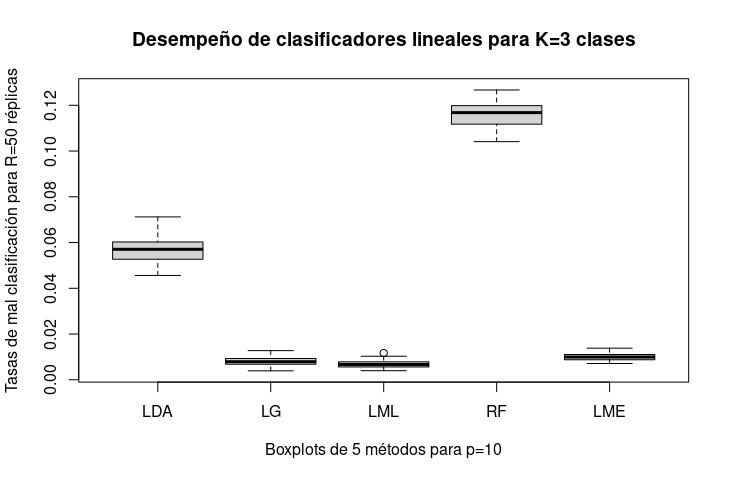
\includegraphics[width=\linewidth]{3_clases_p10_sigma_I}\par 
  		\caption*{$p=10$}
  		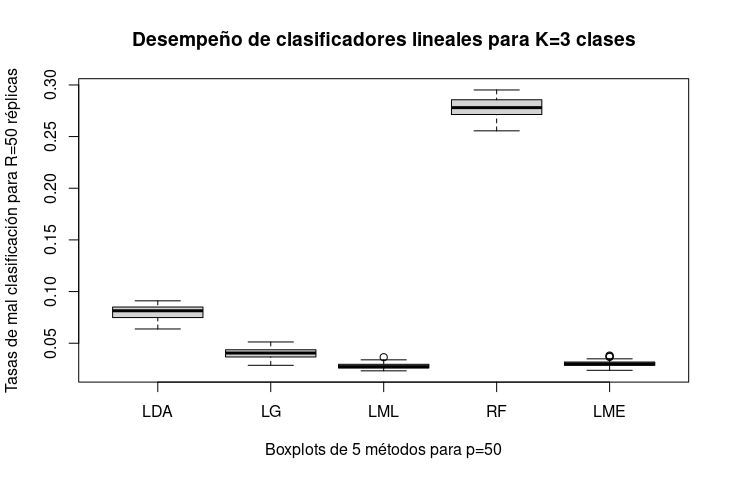
\includegraphics[width=\linewidth]{3_clases_p50_sigma_I}\par 
  		\caption*{$p=50$}	 
  	\end{multicols}
  	\begin{multicols}{2}
  		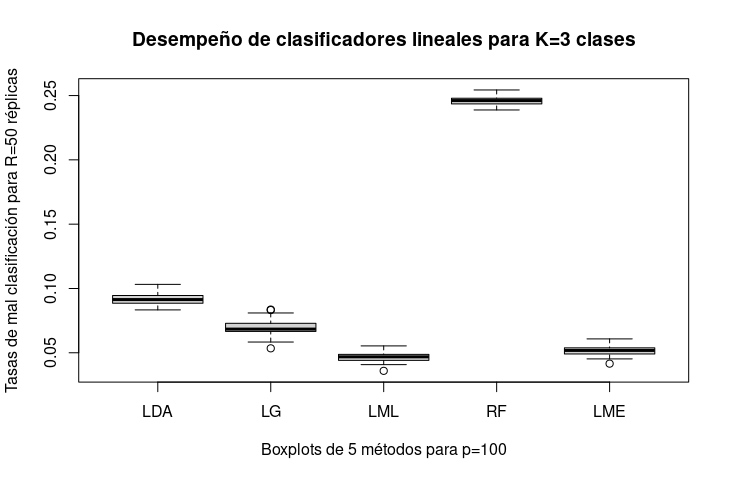
\includegraphics[width=\linewidth]{3_clases_p100_sigma_I}\par
  		\caption*{$p=100$}
  		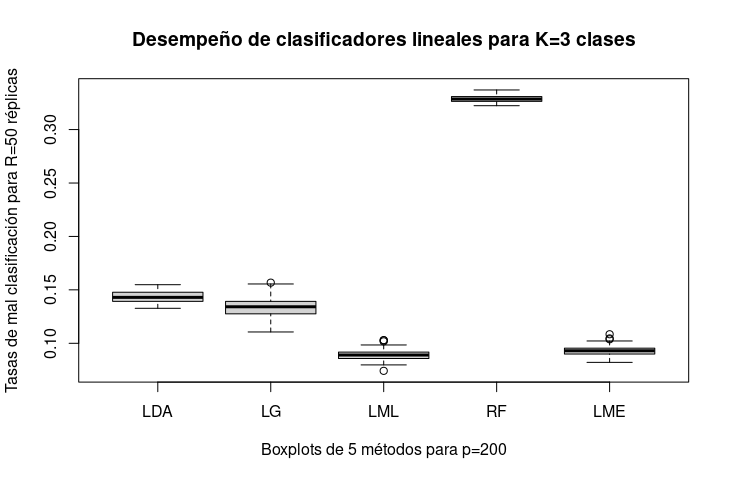
\includegraphics[width=\linewidth]{3_clases_p200_sigma_I}\par 
  		\caption*{$p=200$}
  		
  	\end{multicols}
  	\caption{ Diagramas de caja para la tasa de mala clasificación  a lo largo de $R=50$ réplicas con $K=3$ clases y $\Sigma=I$. }
  	\label{boxk3sigmaiden}
  \end{figure}
  
  \begin{figure} [h]
  	\begin{multicols}{2}
  		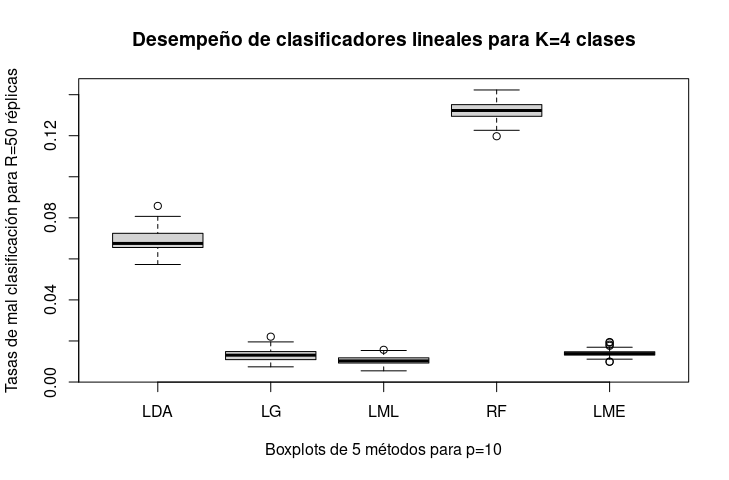
\includegraphics[width=\linewidth]{4_clases_p10_sigma_I}\par 
  		\caption*{$p=10$}
  		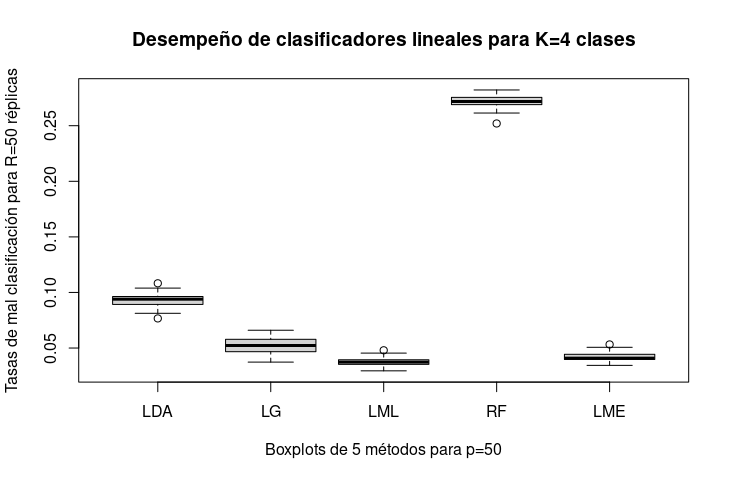
\includegraphics[width=\linewidth]{4_clases_p50_sigma_I}\par 
  		\caption*{$p=50$}	 
  	\end{multicols}
  	\begin{multicols}{2}
  		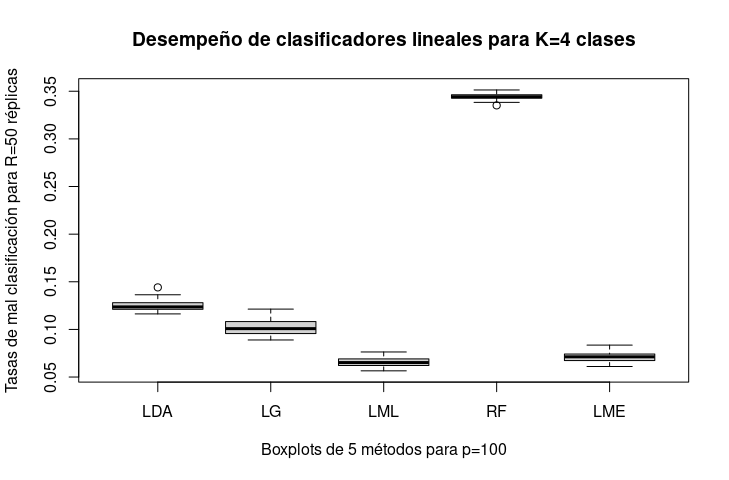
\includegraphics[width=\linewidth]{4_clases_p100_sigma_I}\par
  		\caption*{$p=100$}
  		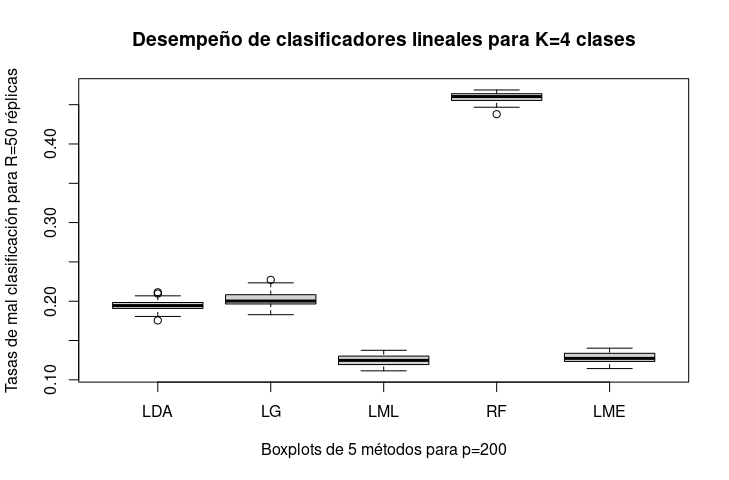
\includegraphics[width=\linewidth]{4_clases_p200_sigma_I}\par 
  		\caption*{$p=200$}
  		
  	\end{multicols}
  	\caption{ Diagramas de caja para la tasa de mala clasificación  a lo largo de $R=50$ réplicas con $K=4$ clases y $\Sigma=I$. }
  	\label{boxk4sigmaiden}
  \end{figure}
  
  
  
  \begin{figure} [h]
  	\begin{multicols}{2}
  		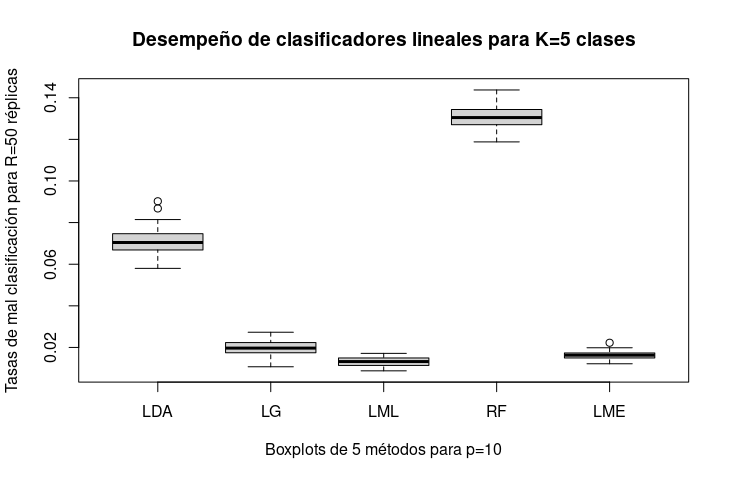
\includegraphics[width=\linewidth]{5_clases_p10_sigma_I}\par 
  		\caption*{$p=10$}
  		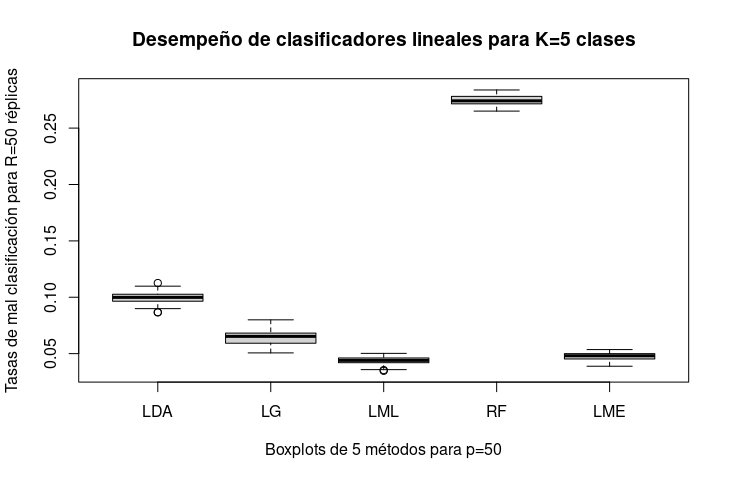
\includegraphics[width=\linewidth]{5_clases_p50_sigma_I}\par 
  		\caption*{$p=50$}	 
  	\end{multicols}
  	\begin{multicols}{2}
  		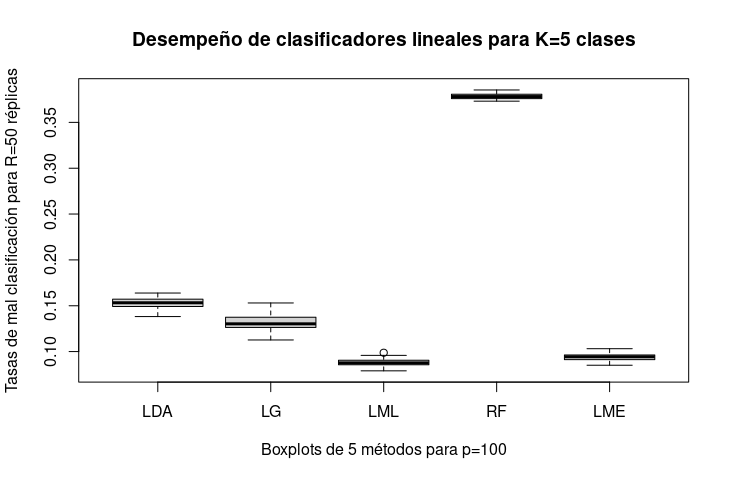
\includegraphics[width=\linewidth]{5_clases_p100_sigma_I}\par
  		\caption*{$p=100$}
  		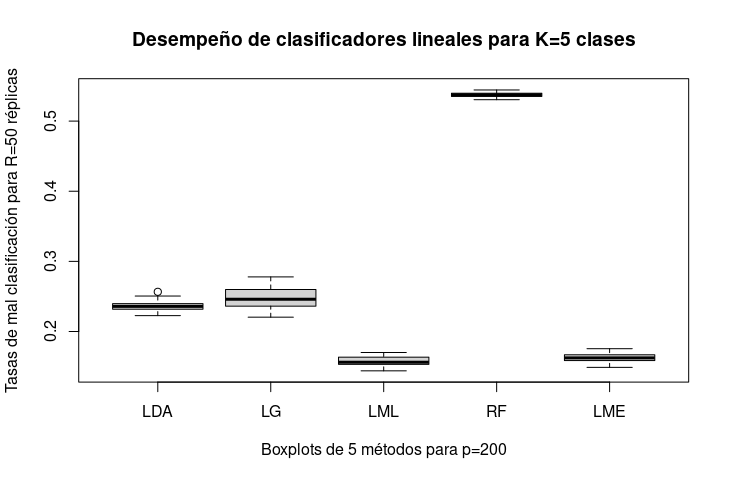
\includegraphics[width=\linewidth]{5_clases_p200_sigma_I}\par 
  		\caption*{$p=200$}
  		
  	\end{multicols}
  	\caption{ Diagramas de caja para la tasa de mala clasificación  a lo largo de $R=50$ réplicas con $K=5$ clases y $\Sigma=I$. }
  	\label{boxk5sigmaiden}
  \end{figure}
  
  
  \begin{figure} [h]
  	\begin{multicols}{2}
  		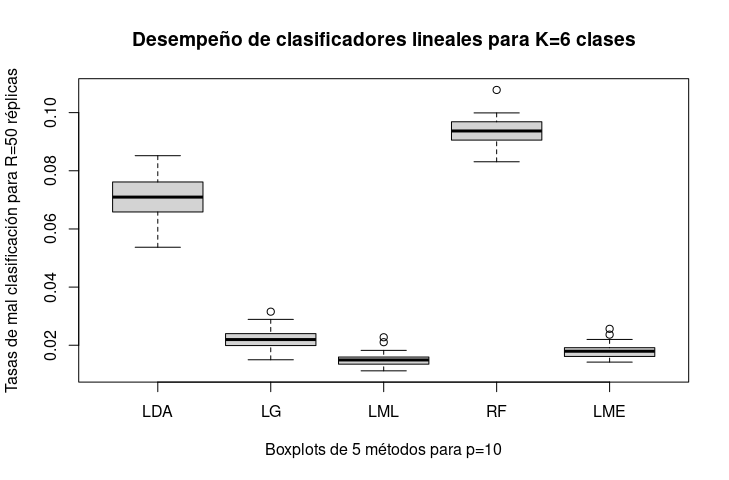
\includegraphics[width=\linewidth]{6_clases_p10_sigma_I}\par 
  		\caption*{$p=10$}
  		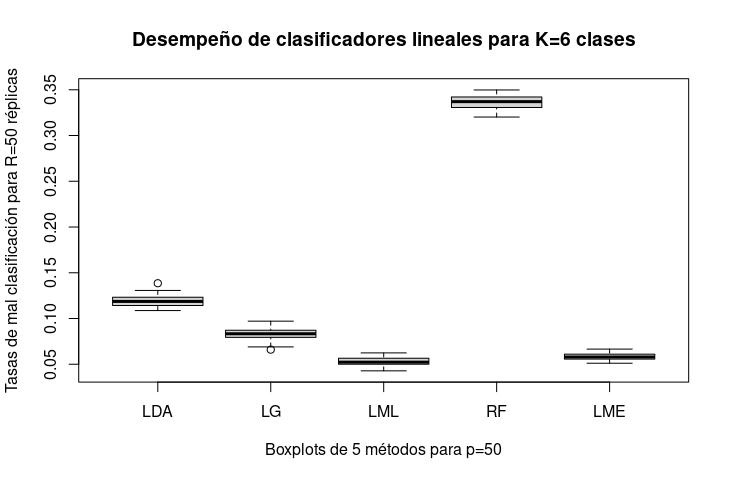
\includegraphics[width=\linewidth]{6_clases_p50_sigma_I}\par 
  		\caption*{$p=50$}	 
  	\end{multicols}
  	\begin{multicols}{2}
  		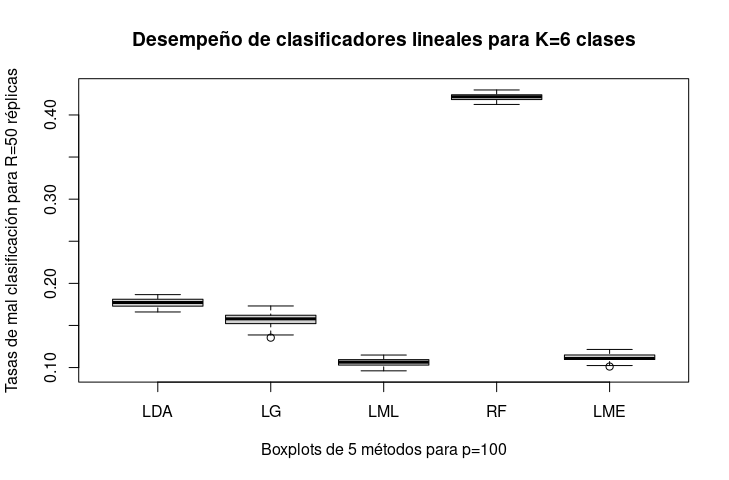
\includegraphics[width=\linewidth]{6_clases_p100_sigma_I}\par
  		\caption*{$p=100$}
  		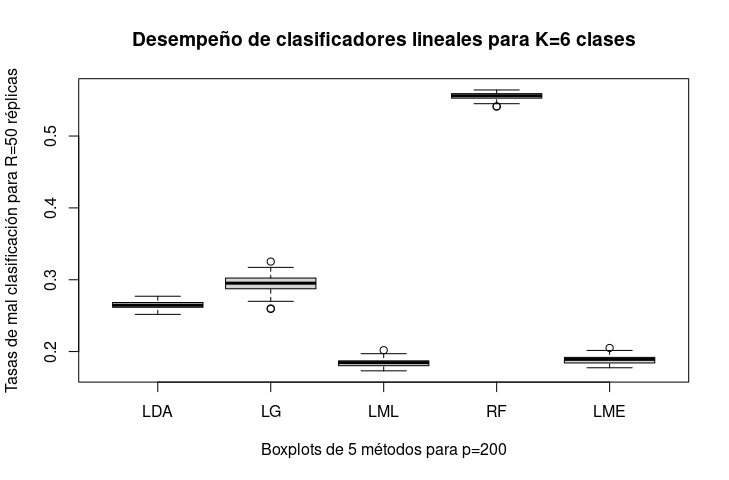
\includegraphics[width=\linewidth]{6_clases_p200_sigma_I}\par 
  		\caption*{$p=200$}
  		
  	\end{multicols}
  	\caption{ Diagramas de caja para la tasa de mala clasificación  a lo largo de $R=50$ réplicas con $K=6$ clases y $\Sigma=I$. }
  	\label{boxk6sigmaiden}
  \end{figure}
  
  \begin{figure} [h]
  	\begin{multicols}{2}
  		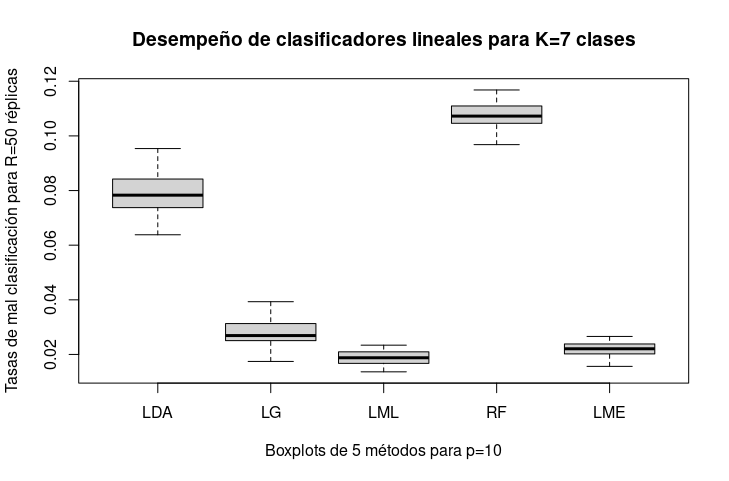
\includegraphics[width=\linewidth]{7_clases_p10_sigma_I}\par 
  		\caption*{$p=10$}
  		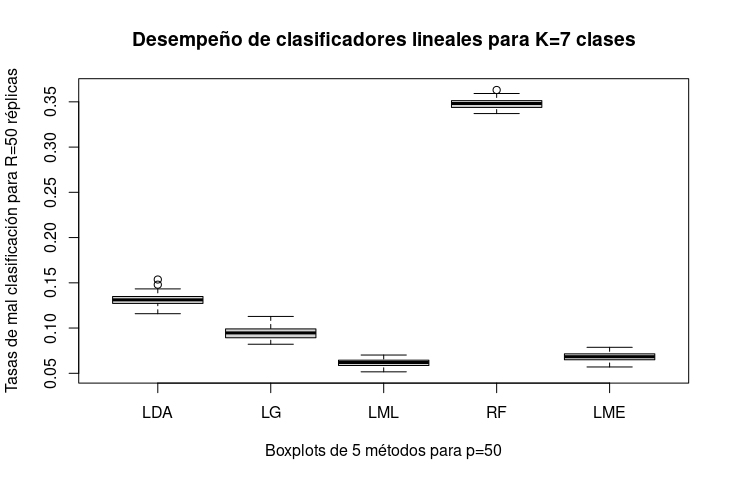
\includegraphics[width=\linewidth]{7_clases_p50_sigma_I}\par 
  		\caption*{$p=50$}	 
  	\end{multicols}
  	\begin{multicols}{2}
  		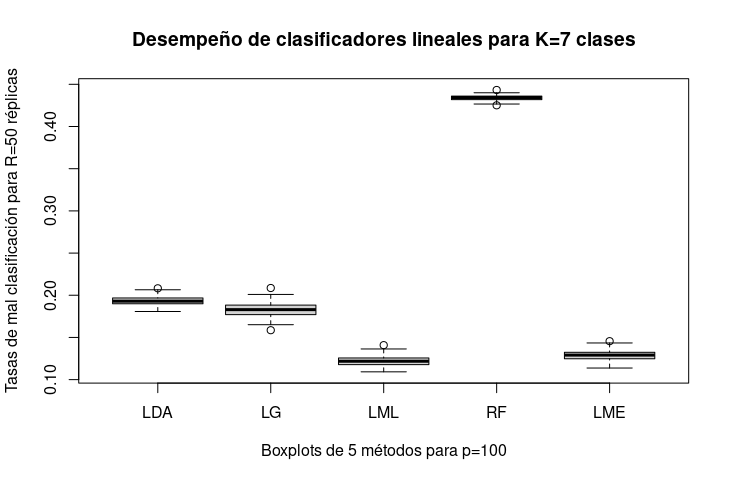
\includegraphics[width=\linewidth]{7_clases_p100_sigma_I}\par
  		\caption*{$p=100$}
  		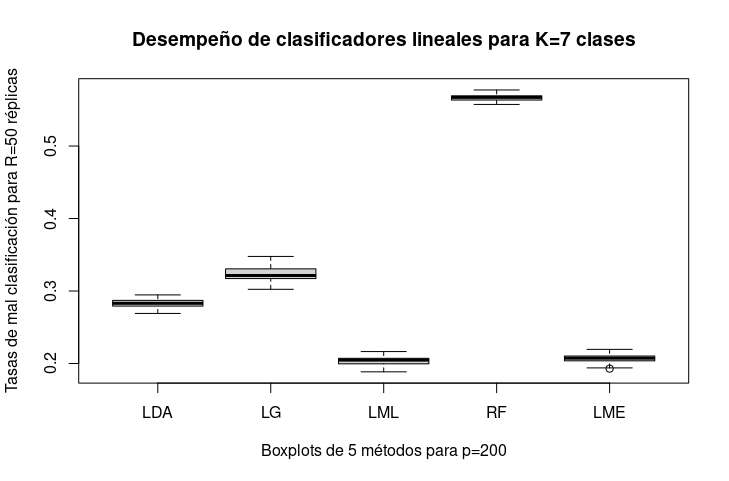
\includegraphics[width=\linewidth]{7_clases_p200_sigma_I}\par 
  		\caption*{$p=200$}
  		
  	\end{multicols}
  	\caption{ Diagramas de caja para la tasa de mala clasificación  a lo largo de $R=50$ réplicas con $K=7$ clases y $\Sigma=I$. }
  	\label{boxk7sigmaiden}
  \end{figure}
  
  
  
  \begin{figure} [h]
  	\begin{multicols}{2}
  		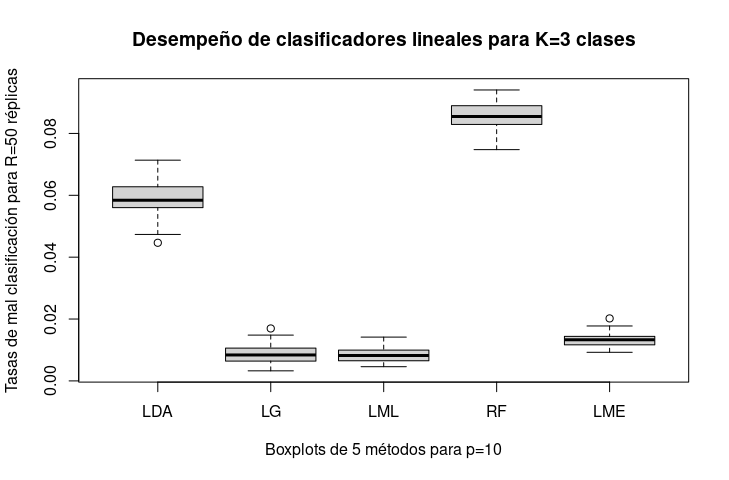
\includegraphics[width=\linewidth]{3_clases_p10_sigma_II}\par 
  		\caption*{$p=10$}
  		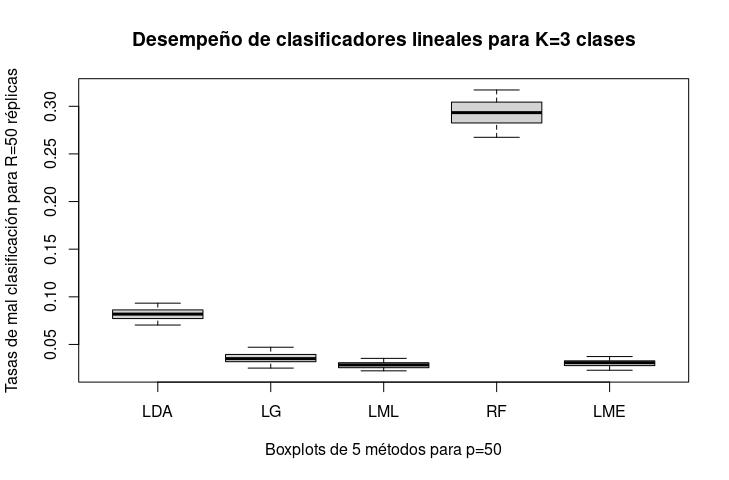
\includegraphics[width=\linewidth]{3_clases_p50_sigma_II}\par 
  		\caption*{$p=50$}	 
  	\end{multicols}
  	\begin{multicols}{2}
  		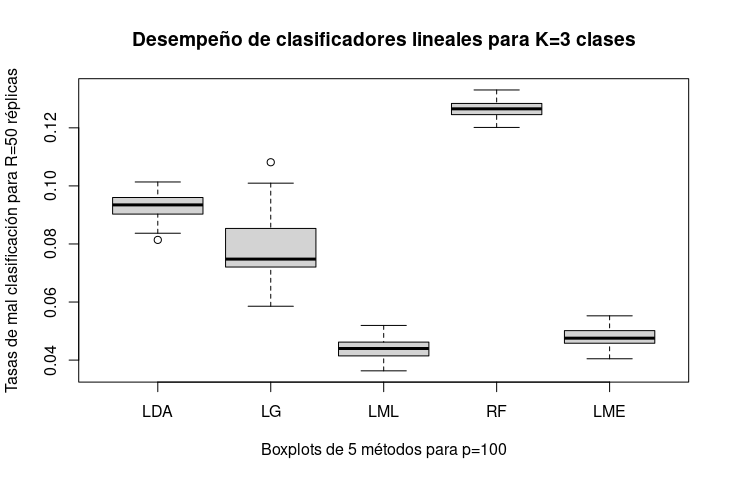
\includegraphics[width=\linewidth]{3_clases_p100_sigma_II}\par
  		\caption*{$p=100$}
  		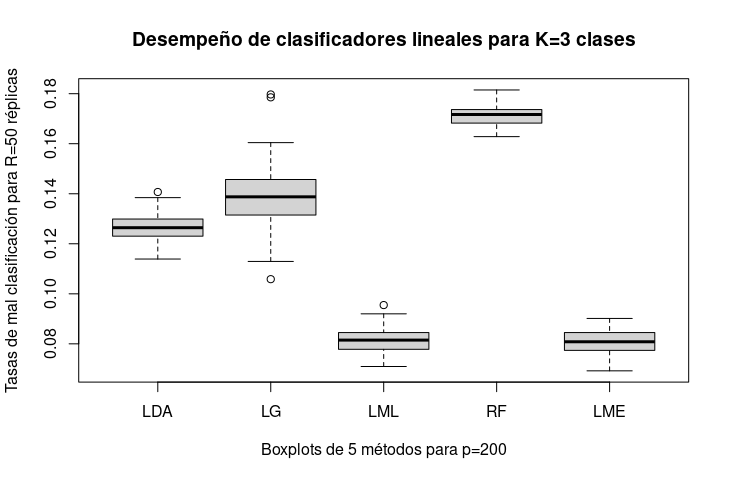
\includegraphics[width=\linewidth]{3_clases_p200_sigma_II}\par 
  		\caption*{$p=200$}
  		
  	\end{multicols}
  	\caption{ Diagramas de caja para la tasa de mala clasificación  a lo largo de $R=50$ réplicas con $K=3$ clases y MAC con $\Sigma=\Sigma_1$. }
  	\label{boxk3alta}
  \end{figure}
  
  \begin{figure} [h]
  	\begin{multicols}{2}
  		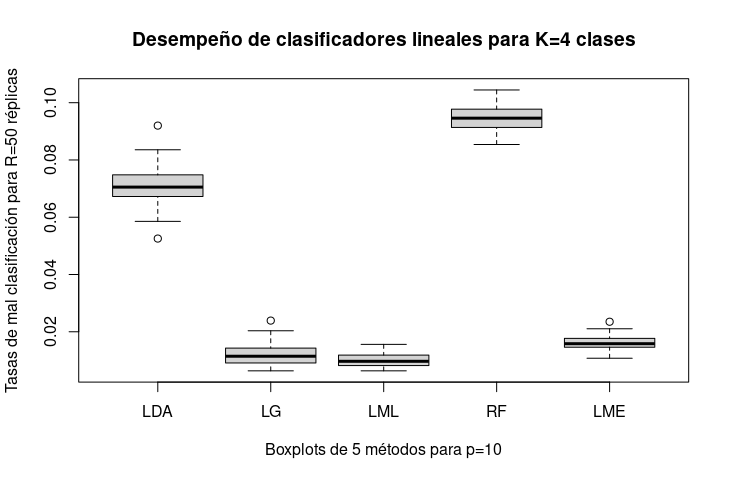
\includegraphics[width=\linewidth]{4_clases_p10_sigma_II}\par 
  		\caption*{$p=10$}
  		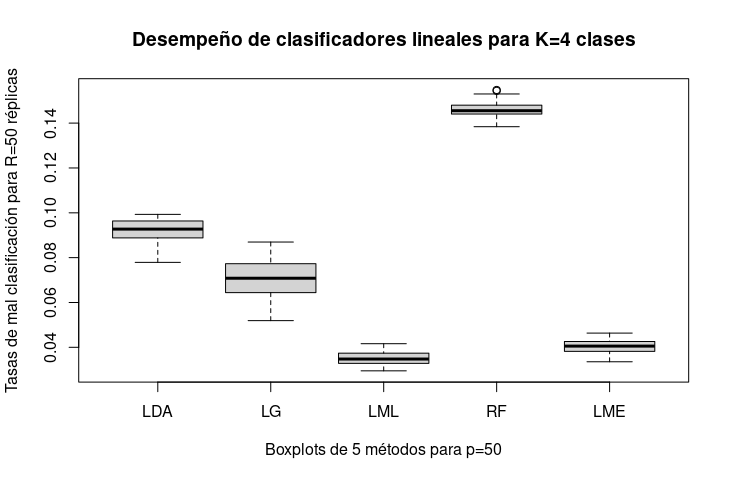
\includegraphics[width=\linewidth]{4_clases_p50_sigma_II}\par 
  		\caption*{$p=50$}	 
  	\end{multicols}
  	\begin{multicols}{2}
  		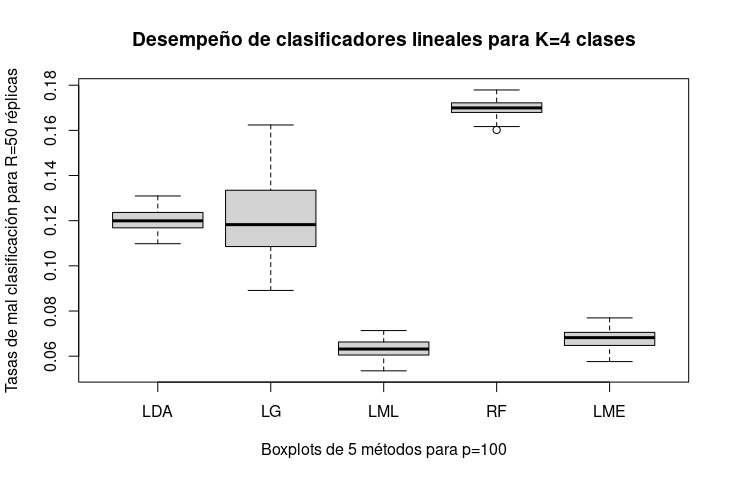
\includegraphics[width=\linewidth]{4_clases_p100_sigma_II}\par
  		\caption*{$p=100$}
  		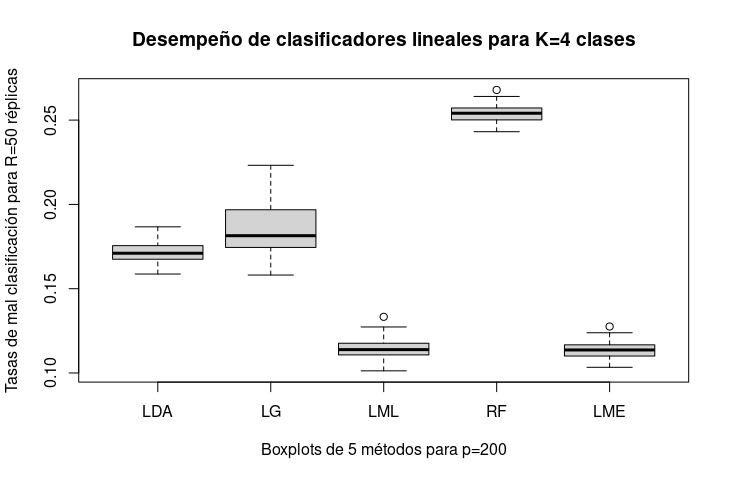
\includegraphics[width=\linewidth]{4_clases_p200_sigma_II}\par 
  		\caption*{$p=200$}
  		
  	\end{multicols}
  	\caption{ Diagramas de caja para la tasa de mala clasificación  a lo largo de $R=50$ réplicas con $K=4$ clases  y MAC con $\Sigma=\Sigma_1$. }
  	\label{boxk4alta}
  \end{figure}
  
  
  
  \begin{figure} [h]
  	\begin{multicols}{2}
  		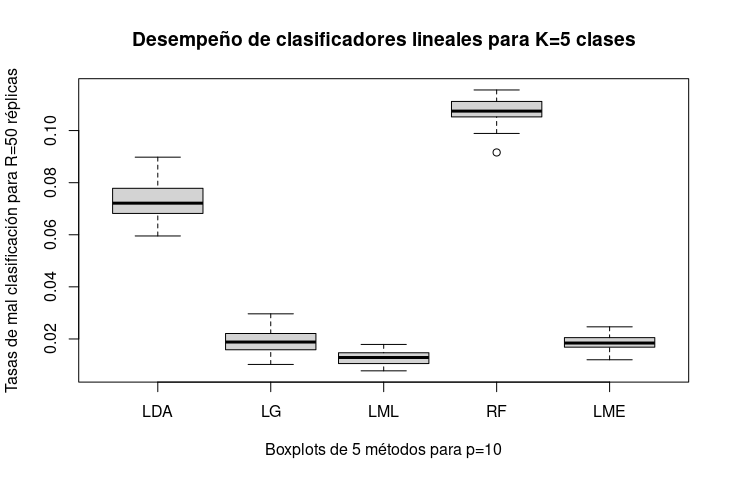
\includegraphics[width=\linewidth]{5_clases_p10_sigma_II}\par 
  		\caption*{$p=10$}
  		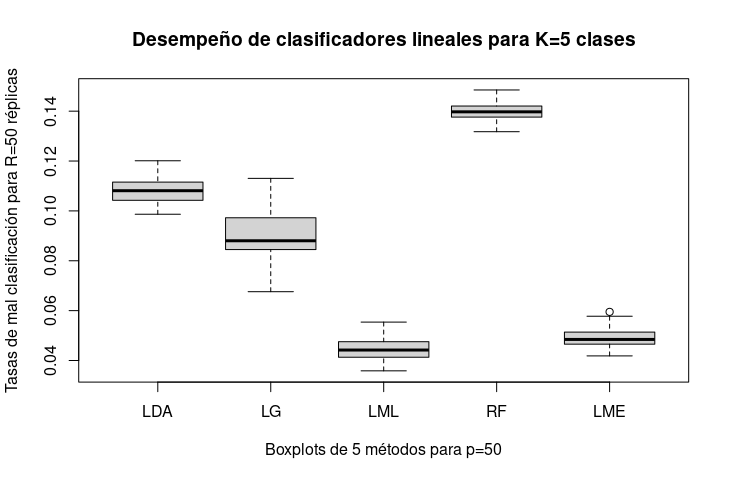
\includegraphics[width=\linewidth]{5_clases_p50_sigma_II}\par 
  		\caption*{$p=50$}	 
  	\end{multicols}
  	\begin{multicols}{2}
  		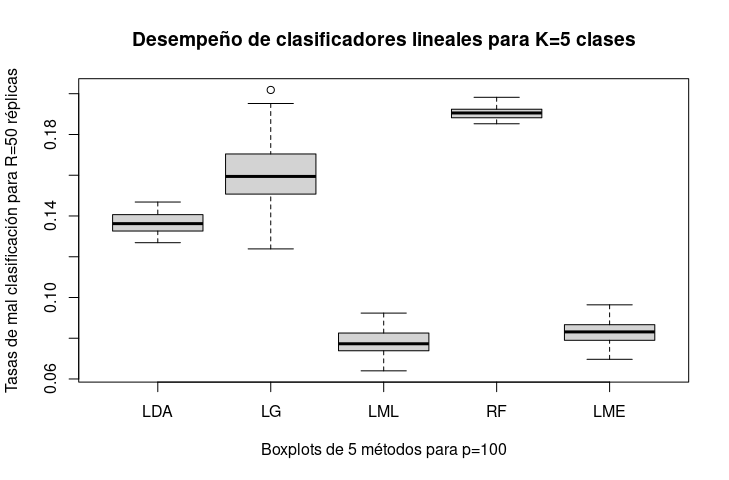
\includegraphics[width=\linewidth]{5_clases_p100_sigma_II}\par
  		\caption*{$p=100$}
  		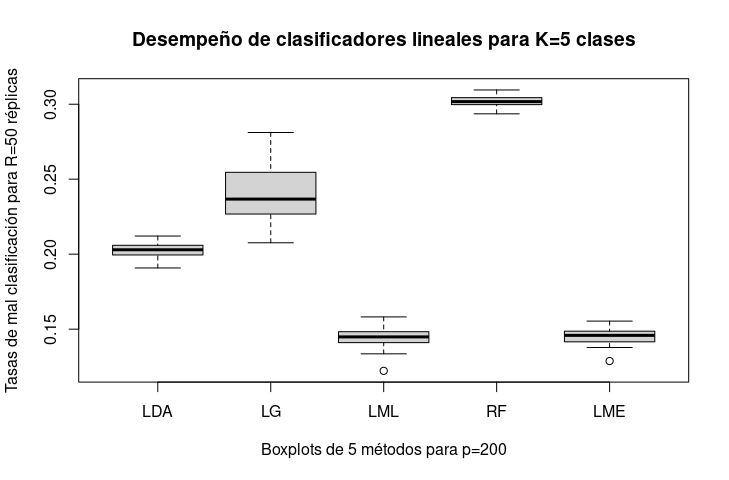
\includegraphics[width=\linewidth]{5_clases_p200_sigma_II}\par 
  		\caption*{$p=200$}
  		
  	\end{multicols}
  	\caption{ Diagramas de caja para la tasa de mala clasificación  a lo largo de $R=50$ réplicas con $K=4$ clases y MAC con $\Sigma=\Sigma_1$. }
  	\label{boxk5alta}
  \end{figure}
  
  
  \begin{figure} [h]
  	\begin{multicols}{2}
  		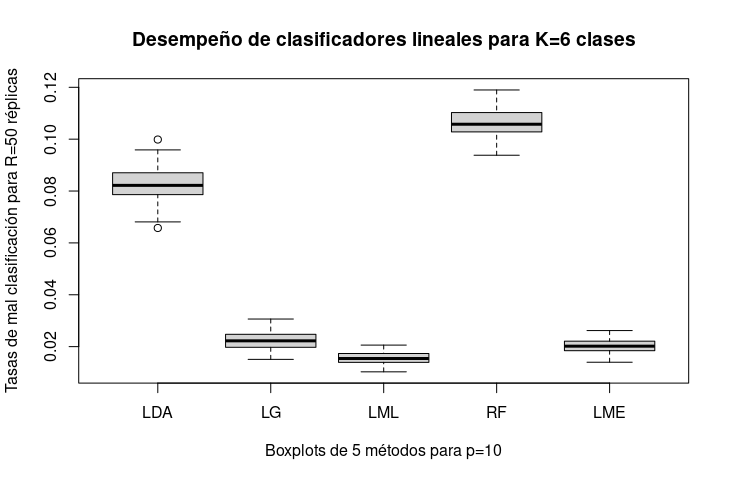
\includegraphics[width=\linewidth]{6_clases_p10_sigma_II}\par 
  		\caption*{$p=10$}
  		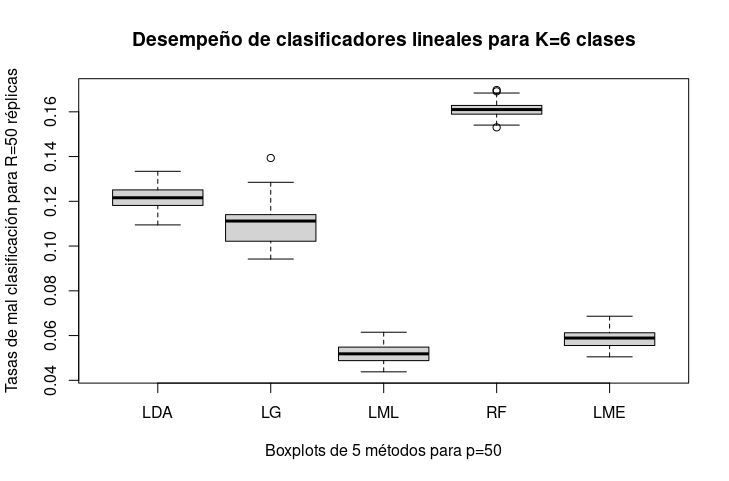
\includegraphics[width=\linewidth]{6_clases_p50_sigma_II}\par 
  		\caption*{$p=50$}	 
  	\end{multicols}
  	\begin{multicols}{2}
  		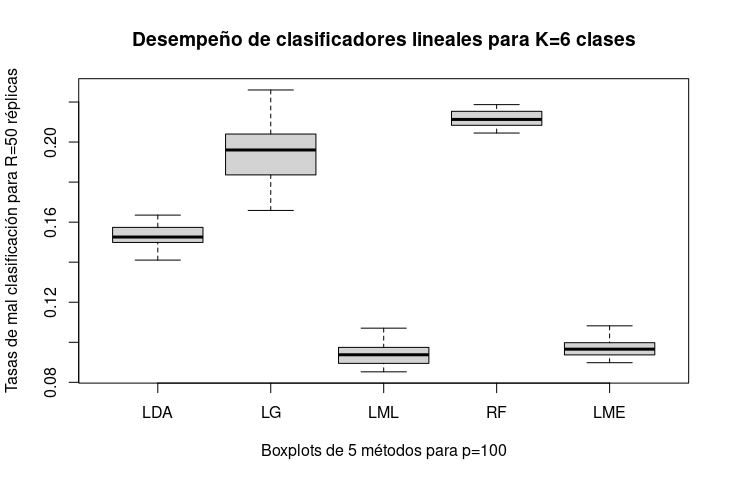
\includegraphics[width=\linewidth]{6_clases_p100_sigma_II}\par
  		\caption*{$p=100$}
  		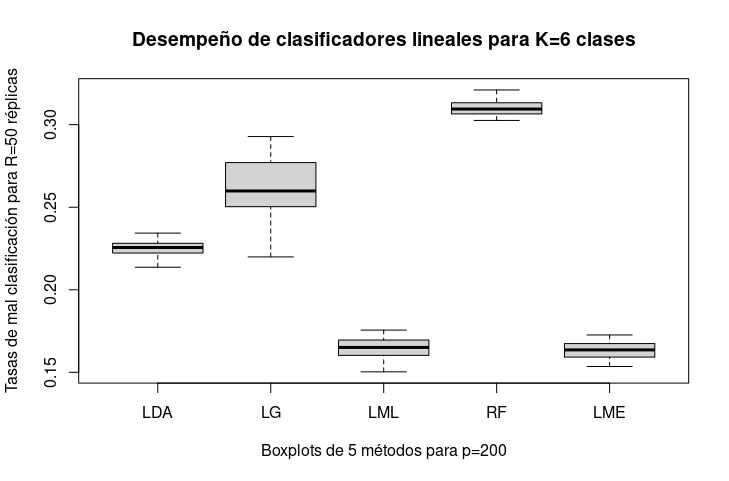
\includegraphics[width=\linewidth]{6_clases_p200_sigma_II}\par 
  		\caption*{$p=200$}
  		
  	\end{multicols}
  	\caption{ Diagramas de caja para la tasa de mala clasificación  a lo largo de $R=50$ réplicas con $K=6$ clases y MAC con $\Sigma=\Sigma_1$. }
  	\label{boxk6alta}
  \end{figure}
  
  
  \begin{figure} [h]
  	\begin{multicols}{2}
  		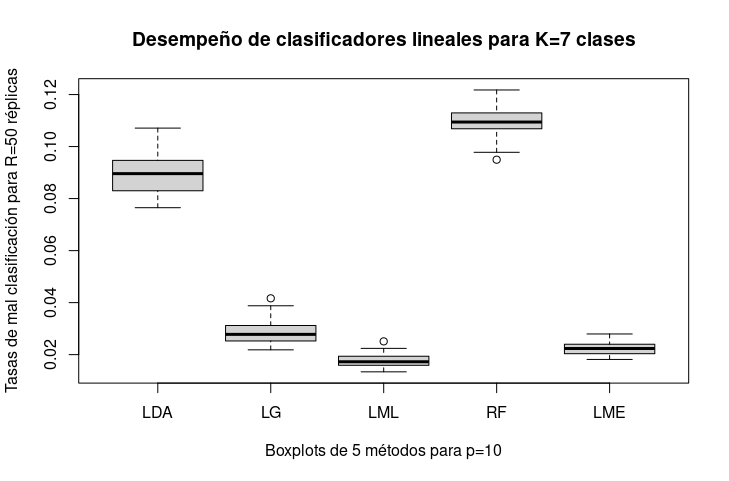
\includegraphics[width=\linewidth]{7_clases_p10_sigma_II}\par 
  		\caption*{$p=10$}
  		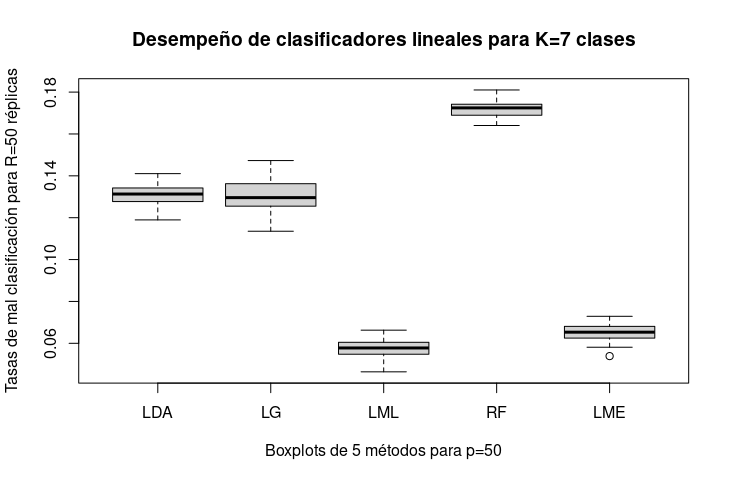
\includegraphics[width=\linewidth]{7_clases_p50_sigma_II}\par 
  		\caption*{$p=50$}	 
  	\end{multicols}
  	\begin{multicols}{2}
  		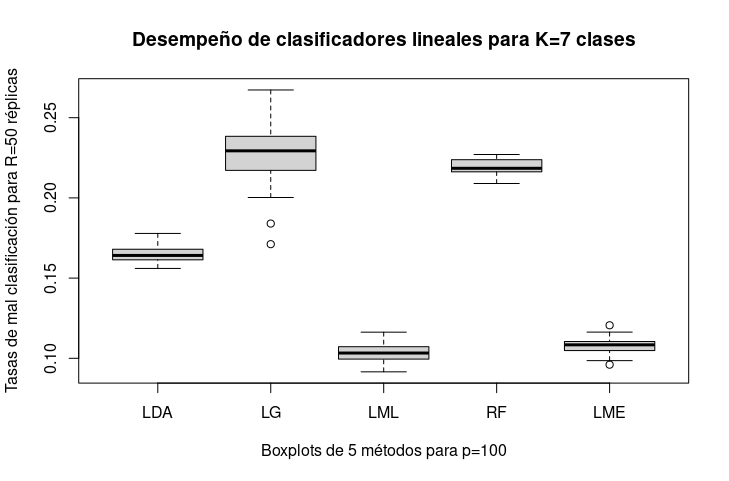
\includegraphics[width=\linewidth]{7_clases_p100_sigma_II}\par
  		\caption*{$p=100$}
  		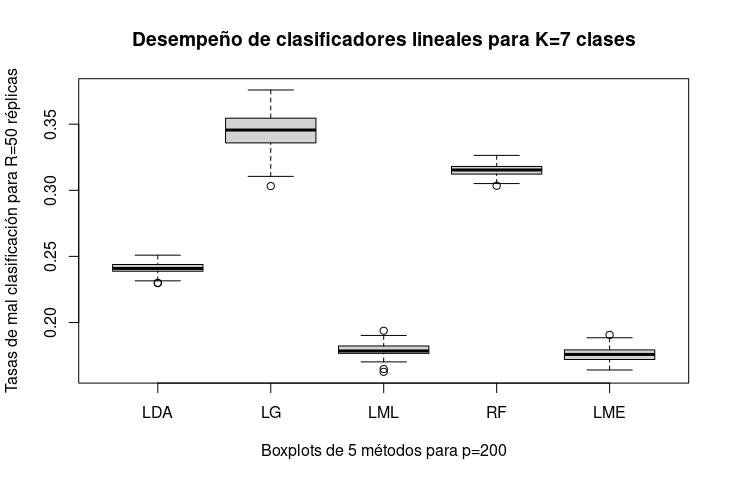
\includegraphics[width=\linewidth]{7_clases_p200_sigma_II}\par 
  		\caption*{$p=200$}
  		
  	\end{multicols}
  	\caption{ Diagramas de caja para la tasa de mala clasificación  a lo largo de $R=50$ réplicas con $K=7$ clases y MAC con $\Sigma=\Sigma_1$. }
  	\label{boxk7alta}
  \end{figure}
  
  




 
\bibliography{bibliografia}
\bibliographystyle{chicago}


\end{document}
